% !TeX spellcheck = en_GB
%===============================================================================
% LaTeX sjabloon voor de bachelorproef toegepaste informatica aan HOGENT
% Meer info op https://github.com/HoGentTIN/bachproef-latex-sjabloon
% 30 bladzijden en 10.000 woorden
%===============================================================================
\documentclass{bachproef-tin}
\usepackage{hogent-thesis-titlepage} % Titelpagina conform aan HOGENT huisstijl
\usepackage{adjustbox}
\usepackage{graphicx}
\usepackage{caption}
\usepackage{subcaption}
\usepackage{listings}

% !TeX spellcheck = en_GB
\newacronym{eol}{EOL}{End Of Life}
\newacronym{it}{IT}{Information Technology}
\newacronym{os}{OS}{Operating System}
\newacronym{hr}{HR}{Human Resources}
\newacronym{vpn}{VPN}{Virtual Private Network}
\newacronym{atp}{ATP}{Advanced Threat Protection}
\newacronym{sdn}{SDN}{Software Defined Networking}
\newacronym{vm}{VM}{Virtual Machine}
\newacronym{wdatp}{WDATP}{Windows Defender Advanced Threat Protection}
\newacronym{roi}{ROI}{Return on Investment}
\newacronym{ws}{WS}{Windows Server}
\newacronym{dtls}{DTLS}{Datagram Transport Layer Security} 
\newacronym{tls}{TLS}{Transport Layer Security} 
%%---------- Documenteigenschappen ---------------------------------------------
% De titel van het rapport/bachelorproef
\title{The migration process and advantages of Windows Server 2019}
% Je eigen naam
\author{Jens Du Four}
% De naam van je promotor
\promotor{Ludwig Stroobant}

% De naam van je co-promotor.
\copromotor{Glenn Verschuere}
% Indien je bachelorproef in opdracht van een bedrijf
\instelling{Delaware}
% Academiejaar
\academiejaar{2018-2019}
% Examenperiode
\examenperiode{2}
%===============================================================================
% Inhoud document
%===============================================================================
\begin{document}
%---------- Taalselectie -------------------------------------------------------
% Als je je bachelorproef in het Engels schrijft, haal dan onderstaande regel
% uit commentaar.
\selectlanguage{english}
%---------- Titelblad ----------------------------------------------------------
\inserttitlepage
%---------- Samenvatting, voorwoord --------------------------------------------
\usechapterimagefalse
% !TeX spellcheck = en_GB
%%=============================================================================
%% Voorwoord
%%=============================================================================

\chapter*{\IfLanguageName{dutch}{Woord vooraf}{Preface}}
\label{ch:voorwoord}

%Throughout the following pages I will research the question: "What are the advantages and disadvantages of a migration from Windows Server 2016 to 2019 in a business environment?". This Bachelors Thesis was written in the context of my graduation at the University College Ghent where I studied Applied Computer Sciences and by order of Delaware, where I researched and wrote my bachelors thesis from February 2019 till May 2019.
%
%In consultation with my promoter, Ludwig Stroobant, and my co-promoter, Glenn Verschuere, the research question was formulated as the basis. For the duration of this assignment, they were always there to answer some of the questions I had in regards to the research that had to be done. 
%
%I would like to thank them in particular. Without them this would not at all have been possible.
%Furthermore I would like to give a special thanks to Delaware and in particular Tomas Castro and Jonas Decoster. Without their effort, I never would have had the opportunity to do this research from their department in China. I would also like to thank Henry Hao for his hospitality and guidance during my stay, it was an experience I will never forget and always be grateful for. 
%
%Finally, I would like to thank my parents in particular. Their wisdom and motivating words have helped me to bring this bachelor's thesis to a successful conclusion.
%
%I wish you a lot of reading pleasure.
%
%Jens Du Four
%
%31/05/2019
%%=============================================================================
%% Samenvatting
%%=============================================================================
%%---------- Nederlandse samenvatting -----------------------------------------
\IfLanguageName{english}{%
\selectlanguage{dutch}
\chapter*{Samenvatting}
Uit een studie is gebleken dat in 2016, {$17.9$}\% en {$45.4$}\% van de servers, in het Spiceworks-netwerk, respectievelijk Windows Server 2003 en Windows Server 2008 gebruikten. \autocite{Tsai2016} 
Deze worden niet langer ondersteund door Microsoft en de uitgebreide ondersteuning voor de laatste loopt ten einde januari 2020. 
Dit betekent dat een grootschalige update naar een nieuwere versie een vereiste wordt voor een aanzienlijk aantal organisaties. 
In deze bachelorproef zijn de voor- en nadelen van een migratie naar Windows Server 2019 onderzocht. 
Er is rekening gehouden met de vier hoofdthema's waarin de nieuwe functies zijn onderverdeeld. 
De migratie tussen de twee versies wordt vervolgens uitgevoerd aan de hand van een in-place upgrade en een side-by-side migratie, met Windows Server 2016 als startpunt. 
Hieruit bleek dat, hoewel een in-place upgrade in een eerste opzicht de eenvoudigste methode is, dit niet altijd de beste is. 
De voordelen van een side-by-side migratie, op vlak van veiligheid en performantie, verantwoorden op lange termijn de additionele inspanning die hiermee gemoeid is.
Aangezien dit \acrshort{os} de basis vormt voor vele applicaties, is ook een migratie van een SAP-omgeving uitgevoerd. 
De SAP Kernel heeft reeds ondersteuning voor Windows Server 2019. 
Een migratie van de gangbare softwareproducten die SAP aanbiedt, is dus mogelijk.
Dit vereist echter bijkomend onderzoek, zoals beschreven in deze bachelorproef. 
Opvallend is dat voor de migratie van andere softwarepakketten eveneens aanvullend onderzoek moet worden verricht. 
Dit om, net als bij Windows Server 2019 en SAP, ervoor te zorgen dat alles voldoet aan de kwaliteitseisen die een organisatie stelt.
Hierna werden de verscheidene beschikbare base container images geanalyseerd. 
Door een verschil in grote en performantie ging de keuze naar de meest recente versie. 
Dit door de additionele functies, die doorheen deze bachelorproef besproken worden, en de toevoeging van de nieuwe Windows base container image.
Tot slot wordt er gekeken naar de toekomst van Windows Server. 
Voornamelijk naar het gebruik van de cloud en de nieuwe functionaliteiten die hiermee gepaard gaan in \acrlong{wac}. 

\selectlanguage{english}
}{}
%%---------- Engelse samenvatting -----------------------------------------------------
\chapter*{\IfLanguageName{dutch}{Samenvatting}{Abstract}}
A study showed that in 2016, {$17.9$}\% and {$45.4$}\% of servers, in the Spiceworks network, respectively used Windows Server 2003 and Windows Server 2008. \autocite{Tsai2016} 
These are no longer supported by Microsoft and the extended support for the latter runs until the end of January 2020. 
This means that a large-scale update to a newer version is becoming a requirement for many organizations. 
In this bachelor's thesis, the advantages and disadvantages of migrating to Windows Server 2019, are investigated. 
The four main themes, in which the new features of Windows Server 2019 are divided, were taken into consideration. 
The migration between both versions is then carried out according to the in-place upgrade and side-by-side migration method, starting from Windows Server 2016. 
This showed that although an in-place upgrade is in first respect the simplest method, it is not always the best. 
The advantages of a side-by-side migration in terms of safety and long-term performance justify the additional effort involved.
Since for many organizations this \acrshort{os} is the basis for their applications, a migration of a SAP environment is also performed. 
The SAP Kernel supports Windows Server 2019. 
A migration of all the trivial software solutions offered by SAP is possible.
However, this requires additional research, as described in this bachelor's thesis.
It is striking that for the migration of other software solutions supplementary research needs to be carried out, as well as additional and rigorous testing. 
This, like done in this bachelor's thesis for Windows Server 2019 and SAP, to ensure that everything meets the quality demands of an organization.
After this, the different available base container images were analysed. 
This showed that because of a difference in size and performance, the choice went to the most recent version. 
This due to the additional functions, which are discussed during this bachelor's thesis and the addition of the new Windows base container image.
Finally, a look is taken at the future of Windows Server. 
Especially at the usage of the cloud and the new functionalities that are paired with this in \acrlong{wac} is taken. 

%---------- Inhoudstafel -------------------------------------------------------
\pagestyle{empty} % Geen hoofding
\tableofcontents  % Voeg de inhoudstafel toe
\cleardoublepage  % Zorg dat volgende hoofstuk op een oneven pagina begint
\pagestyle{fancy} % Zet hoofding opnieuw aan
%---------- Lijst figuren, afkortingen, ... ------------------------------------
% Indien gewenst kan je hier een lijst van figuren/tabellen opgeven. Geef in
% dat geval je figuren/tabellen altijd een korte beschrijving:
%
%  \caption[korte beschrijving]{uitgebreide beschrijving}
%
% De korte beschrijving wordt gebruikt voor deze lijst, de uitgebreide staat bij
% de figuur of tabel zelf.
\listoffigures
\listoftables
% Als je een lijst van afkortingen of termen wil toevoegen, dan hoort die
% hier thuis.
\printnoidxglossaries
%---------- Kern ---------------------------------------------------------------
% De eerste hoofdstukken van een bachelorproef zijn meestal een inleiding op
% het onderwerp, literatuurstudie en verantwoording methodologie.
% Aarzel niet om een meer beschrijvende titel aan deze hoofstukken te geven of
% om bijvoorbeeld de inleiding en/of stand van zaken over meerdere hoofdstukken
% te verspreiden!
% !TeX spellcheck = en_GB
%%=============================================================================
%% Inleiding
%%=============================================================================
\chapter{\IfLanguageName{dutch}{Inleiding}{Introduction}}
\label{ch:inleiding}
Windows Server is an \acrfull{os} that is widely used by organizations all over the world, some with only a handful of employees to corporations that have a couple of thousand at their disposal. 
To keep up in the fast-paced world that is \acrfull{it}, updates are a necessary part of the daily operation, though they do not always present themselves at a convenient time. 
\acrfull{sac} updates which can be scheduled to \acrfull{ltsc} updates, that could require entire systems to be taken offline for an extended duration. 
Since \acrshort{it} has become a core business, this can bring tremendous damage to the business value of many of these organizations.
Therefore, asking how this can be done as efficient and cost-effective as possible is important before considering a migration to the latest version. 

\section{\IfLanguageName{dutch}{Probleemstelling}{Problem statement}}
\label{sec:probleemstelling}
Since the latest version of the Windows Server was released, Windows Server 2019, many organizations are willing to investigate a migration from previous versions of the \acrshort{os} in the nearby future. 
delaware, one of these organizations, wants to research how these migrations would take place starting from Windows Server 2016 and how they can be achieved in an efficient and cost-effective way. 

\begin{table}[htb!]
	\centering
	\begin{adjustbox}{width=1\textwidth}
		\begin{tabular}{l|l|l|ll}
			Products Released & Life Cycle Start Date & Mainstream Support End Date & Extended Support End Date &\\
			\hline
			Windows Server 2016 Standard & 15/10/2016 & 11/01/2022 & 12/01/2027 &\\
			Windows Server 2016 Datacenter & 15/10/2016 & 11/01/2022 & 12/01/2027 &\\
		\end{tabular}
	\end{adjustbox}
	\caption[\acrshort{eol} Windows Server 2016]{\acrlong{eol} of Windows Server 2016}
	\scriptsize	
	Adapted from \cite{MicrosoftEOL2019}
	\label{tab:EOL2016}
\end{table}

With the ending of mainstream support for Windows Server 2016 scheduled at the start of 2022, as seen in Table \ref{tab:EOL2016}, it is best to research the migration to the latest version well in advance. 
Especially when considering that organizations running an \acrfull{eol} \acrshort{os}, are very common. \\
In an article written by \textcite{Tsai2016}, the Spiceworks network showed that the market share of Windows Server 2003 was at {$17.9$}\% and Windows Server 2008 was at {$45.4$}\%. 
The official support for both versions has already ended. 
The extended support for the latter will be ending at the start of 2020. 

\begin{table}[ht]
	\centering
	\begin{adjustbox}{width=1\textwidth}
		\begin{tabular}{l|l|l|ll}
			Products Released & Life Cycle Start Date & Mainstream Support End Date & Extended Support End Date &\\
			\hline
			Windows Server 2019 Essentials & 13/11/2018 & 09/01/2024 & 09/01/2029 &\\
			Windows Server 2019 Standard & 13/11/2018 & 09/01/2024 & 09/01/2029 &\\
			Windows Server 2019 Datacenter & 13/11/2018 & 09/01/2024 & 09/01/2029 &\\
		\end{tabular}
	\end{adjustbox}
	\caption[\acrshort{eol} Windows Server 2019]{\acrlong{eol} of Windows Server 2019}
	\scriptsize	
	Adapted from \cite{MicrosoftEOL2019}
	\label{tab:EOL2019}
\end{table}

Those deadlines combined with the \acrshort{eol} of Windows Server 2016, make a strong case to investigate the migration to the latest version, which can offer enhanced security and additional features. 
The life cycle of the latest version, Windows Server 2019, started in November 2018 and it will continue to receive mainstream support until January 2024. 
The extended support is guaranteed until January 2029, as seen in Table ~\ref{tab:EOL2019}.\\
This makes it a viable successor for the \acrshort{os} that makes up a large percent of the server infrastructure used in the world. 
This bachelor's thesis attempts to show that the benefits that are paired with migrating will outweigh the disadvantages. 
The new features of the latest version can be divided into four key themes \autocite{MWST2018}:

\begin{itemize}
	\item Hybrid cloud
	\item Security
	\item Application platform
	\item Hyper-converged infrastructure
\end{itemize}

Those four themes will be examined thoroughly in Chapter \ref{ch:stand-van-zaken}.

\section{\IfLanguageName{dutch}{Onderzoeksvraag}{Research question}}
\label{sec:onderzoeksvraag}
What are the advantages and disadvantages of a migration from Windows Server 2016 to Windows Server 2019 in a business environment?

\subsection{Sub-research question}

\begin{itemize}
	\item What are the differences between the Windows, Server Core and Nano Server base container images of Windows Server 2019?
	\item Can SAP be migrated from an existing Windows Server 2016 to Windows Server 2019 in a business environment?
	\item How can the new features of Windows Server 2019 be leveraged in the migrated infrastructure? 
\end{itemize}

\section{\IfLanguageName{dutch}{Onderzoeksdoelstelling}{Research objective}}
\label{sec:onderzoeksdoelstelling}

The expected result of this bachelor's thesis is to demonstrate the advantages of utilizing Windows Server 2019 over Windows Server 2016, proving that migration is a long-term investment towards the future for any organization. 
It will also compare the base container images of the \acrshort{os} and show that a migration of a SAP environment to Windows Server 2019 can be done. 
This because the  requirements between the latest version of both the \acrshort{os} and the SAP Kernel have been met. 

\section{\IfLanguageName{dutch}{Opzet van deze bachelorproef}{Structure of this bachelor's thesis}}
\label{sec:opzet-bachelorproef}

The remainder of this bachelor's thesis is structured as follows:

In Chapter ~\ref{ch:stand-van-zaken}, an overview is given of the state of the art within the research domain, based on a literature study.
\\

In Chapter ~\ref{ch:methodologie}, a methodology is explained, and the research techniques used to formulate an answer to the research questions are discussed.
\\

In Chapter ~\ref{ch:toekomstvisie}, the further development of Windows Server over the years to come will be analysed. 
\\

In Chapter~\ref{ch:conclusie}, finally, the conclusion is given, and an answer is formulated to the research questions. This will also provide an impetus for future research within this domain.
\\

% !TeX spellcheck = en_GB
\chapter{\IfLanguageName{dutch}{Stand van zaken}{State of the art}}
\label{ch:stand-van-zaken}
% Tip: Begin elk hoofdstuk met een paragraaf inleiding die beschrijft hoe dit hoofdstuk past binnen het geheel van de bachelorproef. Geef in het bijzonder aan wat de link is met het vorige en volgende hoofdstuk.
In this chapter the state of affairs will be examined. As mentioned in the introduction, this part of the bachelor's thesis will be used to get an in-depth understanding of the four key themes that incorporate the changes in Windows Server 2019. First, for the key themes mentioned before, a basic understanding of what they are will be established together with how these have been implemented in the latest version of the \acrshort{os}.

\section{Hybrid cloud}
Hybrid Cloud is a topic that has gained more momentum over the past years. For organizations, this makes it a consistent topic of interest and makes it one of the keystone themes in Windows Server 2019. \autocite{MWST2018} It is with this in mind that it is discussed as an essential part of the bachelor's thesis. It is especially beneficial to know the advantages that this aspect offers to Windows Server since the latest version, how these improve workflow and how they can be leveraged by organizations, in particular, Delaware. To start with, the different types of clouds will be analysed and discussed in the following subsection.

\subsection{Types of cloud solutions}
The National Institute of Standards and Technology differentiates four types of clouds \autocite{Mell2011}:
\begin{itemize}
	\item Private Cloud
	\item Community Cloud
	\item Public Cloud
	\item Hybrid Cloud
\end{itemize}	
It is  however important to keep in mind that virtualization is not the same as cloud computing. While virtualization detaches computing environments from their physical infrastructure through software, cloud computing is a service that delivers computing resources on demand via a network. \autocite{Naeem2016}

\subsubsection{Private cloud}
A private cloud is an internal infrastructure in the cloud that is designated for usage by a single organization. It can however consist of multiple clients, albeit in the same organization. It is only accessible inside a private internal network or over the Internet for a selected amount of users than for the public. Private clouds can also be known by other names such as internal or corporate cloud. Their main advantage is the higher level of security and privacy . They offer this to organizations through the usage of in-house hosted infrastructure and additional company firewalls. The biggest disadvantage that comes with this added layer of security is the responsibility that is given to the \acrfull{it} team that manages the infrastructure that supports the private cloud. This means, on top of the additional in-house hosting cost, that they require the same amount of man-hours that come with the management of a traditional data centre. Keep in mind that in-house does not necessarily mean on-premise.
Still, the private cloud holds a great benefit compared to long-standing methods. As reported by IBM, an organization that saved more than \$1.5 billion by reducing their number of datacenters from 115 to 5. This was a direct result of the implementation of a private cloud. \autocite{Hofmann2010} 


\subsubsection{Community cloud}
When several organizations collaborate to meet the requirements that are demanded of the \acrshort{it} infrastructure, they are operating under a community cloud. This means that it can be managed in-house or by a third-party organization that operates inside the same community. This form of operation tackles one of the main problems of a private cloud. It shares the costs over multiple organizations, thus greatly reducing it for a single organization. Since they are operating inside the same community, they share the same concerns and will be subjected to the same requirements that can be imposed by a governing instance. 
This advantage over private clouds is only a partial improvement. This cost reduction as a result of sharing the infrastructure means a devaluation of security. Meaning that it is a viable alternative to  organizations that have some security concerns with the usage of a public cloud, but are willing to make some sacrifices in favour of lower costs. 
\newline
An example of this is described in an article \autocite{Yao2014} about how small hospitals in China, not all of which can provide their own infrastructure, could utilize a community cloud. These grass-roots healthcare institutions, that all operate within the same community, can share the cost and management of the cloud to provide an attractive hospital information solution to improve their service without the extensive cost nor the need for additional security concerns regarding confidential information in patient files.

\subsubsection{Public cloud}
Amazon Web Services, Oracle Cloud and Microsoft Azure are only some examples of public clouds. Most of these solutions are offered by corporations, like those mentioned above, who manage and operate their data centres and provide access to their cloud via the Internet. Thus eliminating the cost that is associated with the management and responsibility of a private cloud, where the \acrshort{it} department is responsible, and so significantly reduces the cost in equivalent use cases. Public clouds also provide the possibility for painless scalability and flexibility in comparison with private clouds, in which the hardware needs to be available in-house. This makes the public cloud ideal for temporary solutions.
\newline
\textcite{Singh2012} concluded, in a comparison between the cost and security of private and public clouds over three years, that although security can be a real concern in the usage of public cloud it should not be ruled out immediately without fully analysing the requirements of an organization, this with keeping in mind the major investment that comes paired with the usage and implementation of a private cloud.  
The different obstacles that securing a public cloud has are also addressed by \textcite{Ren2012}, in which there is a call for additional research about the subject to fully take advantage of the revelation that cloud computing is. 

\subsubsection{Hybrid cloud}
A hybrid cloud aims to be the solution for every business. It combines the higher level of security and privacy that is offered by the private cloud with easy scalability and flexibility that comes paired with the public cloud. In a hybrid cloud the organization manages a part of its cloud infrastructure in-house and a part out-house. As described in the book by \textcite{Sarna2010}, hybrid clouds enables large organizations to move their less sensitive information, like \acrfull{hr}, to the cloud. Thanks to the advantages of hybrid cloud their sensitive data, such as classified information about costumers or the organization, can remain in-house on private clouds or even on-premise for an additional layer of security. The connection between both the public and private cloud part of the hybrid cloud is generally accomplished through a \acrfull{vpn}.

\subsection{Hybrid cloud in Windows Server 2019}
%TODO Windows Admin Center

\section{Security}
With more than 53.000 reported incidents and 2.216 confirmed data breaches \autocite{Verizon2018}, security has become an essential part of \acrshort{it}. The importance of security directly translates into Windows Server 2019 through various parts of the \acrshort{os} that have either been reviewed to make them more resilient and accessible or new features which have been added to further improve security. In the following section all the major elements will be discussed, distributed among three subsections:
\begin{itemize}
	\item Windows Defender \acrfull{atp}
	\item Security with \acrfull{sdn}
	\item Shielded Virtual Machines
\end{itemize}

\subsection{Windows Defender \acrfull{atp}}
In a research study done by \textcite{Musto2017} \acrfull{wdatp} was scrutinized. When the endpoint security solution is implemented in Windows Server 2019, it requires additional licensing. Still, the efficiency with which it tackles security problems resulted in a 53\% \acrfull{roi}. The research reported that \acrshort{wdatp} reduced the risk of a breach by 40\%. It even enabled them to identify threats faster and resolve them in a more efficient fashion. In conclusion, the replacement of previous solutions with \acrlong{wdatp} reduced costs and made security teams more efficient. With the advent of Windows Server 2019, additional features have been added to \acrlong{wdatp} to ensure the safety of organizations in the years to come. The different components of \acrshort{wdatp} are described in the picture below. Those will not be individually reviewed here as this subject alone offers enough content for another bachelor's thesis.
\begin{figure}[hbt!]
	\centering
	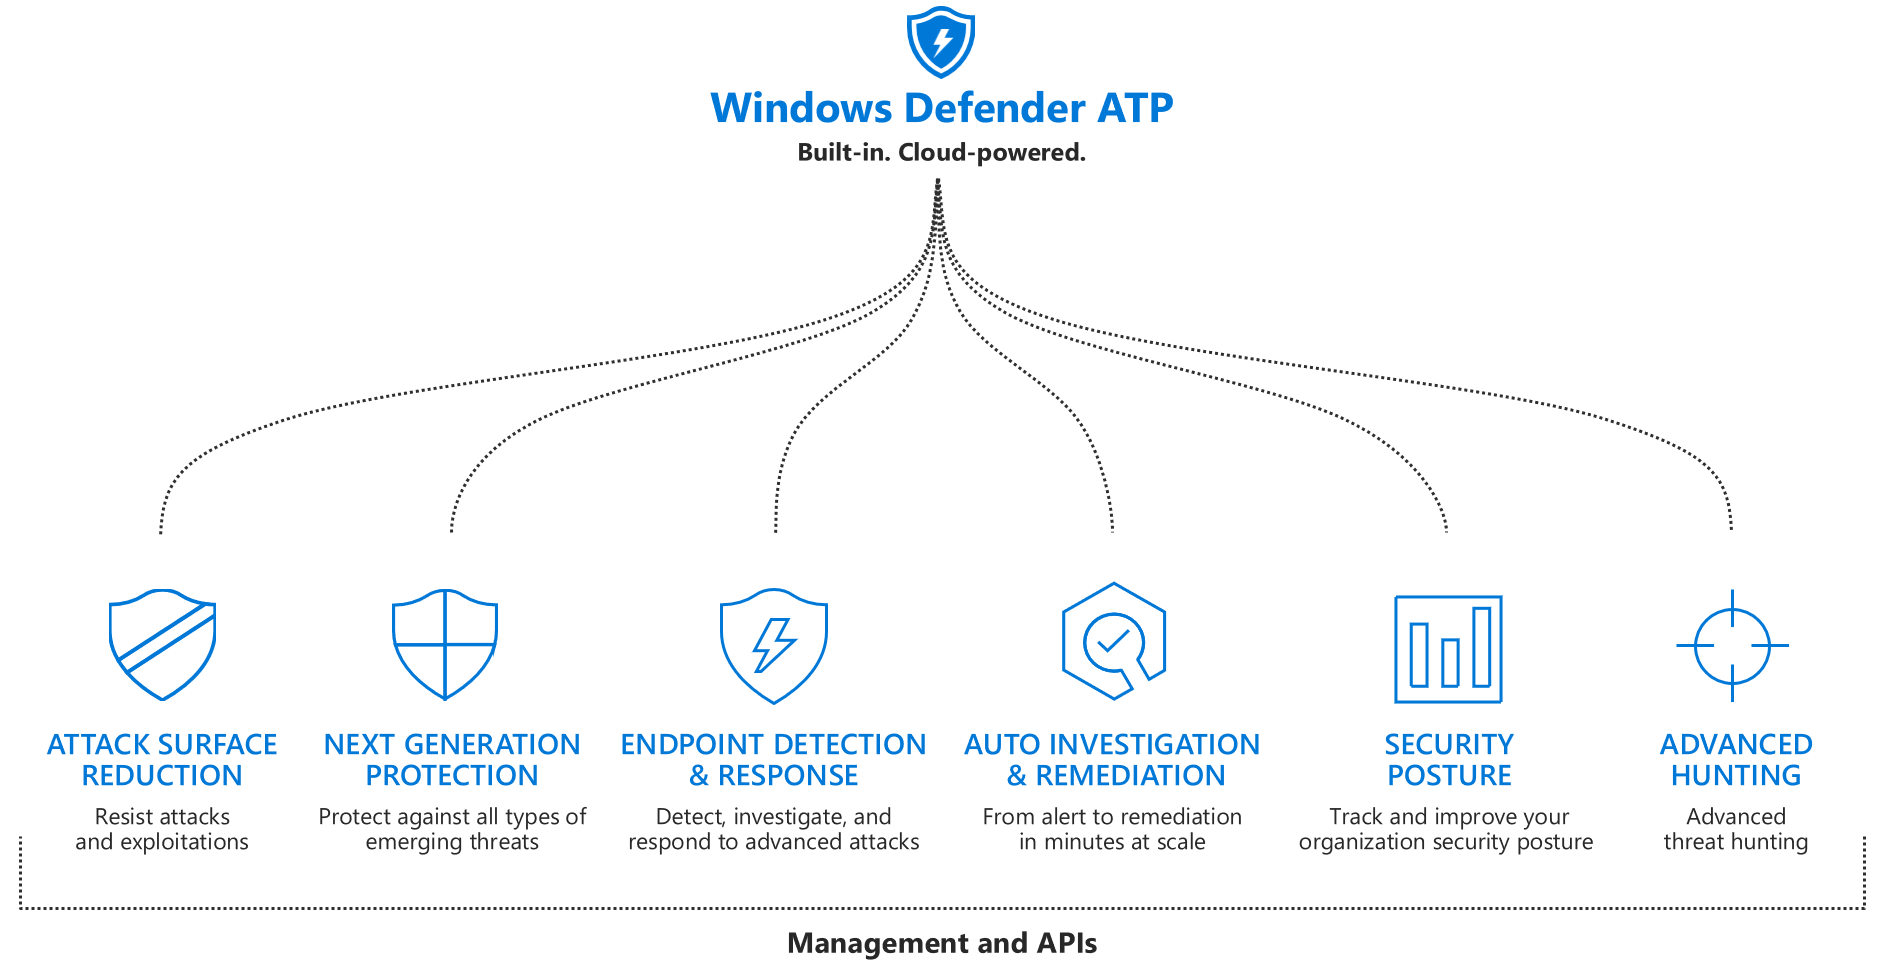
\includegraphics[width=\textwidth,height=6cm,keepaspectratio=true]{img/Windows-Defender-ATP.png}
	\caption[Components of \acrshort{wdatp}]{The different components of \acrlong{wdatp}. \autocite{Aslaner2018}}
	\label{fig:WDATPT2018}
\end{figure}

\subsection{Security with \acrfull{sdn}}
As described by \textcite{Shin2016}, \acrfull{sdn} is a state-of-the-art technology that enables developers to design advanced networks effortless. In Windows Server 2019 their have also been new development in this field, these can be boiled down to four features. The discussion of these will be constrained.
\begin{itemize}
	\item Encrypted networks
	\item Firewall auditing
	\item Virtual network peering
	\item Egress metering
\end{itemize} 

\subsubsection{Encrypted networks}
Encrypted networks, or more specifically virtual encrypted networks, enable the encryption of network traffic between different \acrlong{vm}s. It does this through the usage of \acrfull{dtls}. \acrshort{dtls} was built as close to \acrshort{tls} as possible \autocite{Modadugu2004}, which makes it ideal at securing connections. However, for the connection between \acrlong{vm}s \acrshort{dtls} is preferred, since these connections are delay sensitive. 

\subsubsection{Firewall auditing}
One of the new features in Windows Server 2019 is \acrshort{sdn} Firewall auditing. This means that the administrator is enabled to see if every part of his Firewall is as secure as is initially thought. When this feature is enabled every data stream that gets processed by the \acrshort{sdn} firewall, gets recorded. The logs can than be used in troubleshooting or archived for analysis. These can also be processed by using tools such as Power BI.

\subsubsection{Virtual network peering}
Virtual network peering allows you to combine two individual virtual networks. A coherent connection is made that represents itself as an individual one. This means the connection between both networks can be routed through the infrastructure backbone, this in term means that there is no need for a public gateway. Providing a more secure connection, while no additional downtime is accumulated when peering the networks.

\subsubsection{Egress metering}
Egress metering for \acrshort{sdn} enables an administrator to monitor the consumption on outgoing connections. Windows Server 2019 also makes a distinction between traffic that leaves the virtual network and the data centre, in comparison to traffic that stays within the data centre. 

\subsection{Shielded Virtual Machines}
One of the requirements to run a Shielded \acrfull{vm} is a \acrfull{hgs}. Since Windows Server 2019 it is possible to run Shielded \acrshort{vm}s on machines with irregular connection to the \acrshort{hgs}. This can be done by leveraging the two new features. 

\begin{description}
	\item[Fallback \acrshort{hgs}] Provide a redundant connection in case the primary \acrshort{hgs} can not be reached.
	\item[Offline Mode] Once a shielded \acrshort{vm} has been setup it can be started up seeing the security configuration remains unchanged.
\end{description}

Another new feature is the addition of support for Ubuntu, Red Hat Enterprise Linux and SUSE Linux Enterprise Servers inside Shielded \acrshort{vm}s. 

\section{Application platform}
% TODO Application Platform
%\subsection{Linux containers on Windows}
%\subsection{Building Support for Kubernetes}
%\subsection{Container improvements}
%\subsection{Encrypted Networks}
%\subsection{Network performance improvements for virtual workloads}
%\subsection{Low Extra Delay Background Transport}
%\subsection{Windows Time Service}
%\subsection{High performance SDN gateways}
%\subsection{New Deployment UI and Windows Admin Center extension for SDN}
%\subsection{Persistent Memory support for Hyper-V VMs}

\section{Hyper-converged infrastructure}
% TODO HCI
\section{Conclusion}
% TODO Conclusion
% !TeX spellcheck = en_GB
%%=============================================================================
%% Methodologie
%%=============================================================================
\chapter{\IfLanguageName{dutch}{Methodologie}{Methodology}}
\label{ch:methodologie}
In this chapter, the migration from Windows Server 2016 to Windows Server 2019 will be executed. 
This migration will first be performed on an environment which has been based on the Modern Desktop Deployment and Management Lab Kit provided by Microsoft. \autocite{Gallagher2018} 
Here a \acrfull{dc} will be migrated. 
After this, the migration of a typical SAP environment, as described by delaware, from Windows Server 2016 to Windows Server 2019, will be performed. 
Finally, the different versions of the Windows Server 2019 base container images will be analysed. 
How these can lower virtual machine overhead and improve virtualization efficiency compared to their predecessor, will be reviewed. 
But first, the infrastructure that was used for the initial migration will be discussed.

\section{Migrating the \acrshort{os}}
\label{sec:Migrating_the_OS}
In this section, a \acrshort{dc} will be migrated using both the in-place upgrade and side-by-side migration method. 
This to show the basics of the migration process in an environment where no third-party services, such as SAP, are running. 
That will be discussed in Section \ref{sec:SAP}.

\subsection{Technical specifications of the proof of concept environment}
The proof of concept was made using a bare-metal server, running Windows Server 2016. 
The proof of concept environment was than virtualized using Hyper-V. 
Additionally, \acrlong{wac} was also installed locally, this to make the management of the resources easier and more efficient.
The specifications of the server are the following:

\begin{itemize}
	\item CPU: Intel Xeon E5620
	\item RAM: 96 GB 
	\item HDD: 500 GB
	\item OS Version: Windows Server 2016
	\item Hyper-V role installed
	\item Administrative rights on the device
\end{itemize}

The proof of concept environment was based on the Modern Desktop Deployment and Management Lab Kit provided by Microsoft. \autocite{Gallagher2018}
This to make replication of the environment simple and efficient.
\\
The Modern Desktop Deployment and Management Lab Kit consists of the components in Table \ref{tab:LKC}.
\\

\begin{table}[ht]
	\centering
	\begin{adjustbox}{width=1\textwidth}
		\begin{tabular}{l|l}
			Server Name  & Roles \& Products                                                  	 \\ 
			\hline
			HYD-DC1      & Active Directory Domain Controller, DNS, DHCP, Certificate Services 	   \\
			HYD-MDT1     & Microsoft Deployment Toolkit                                        		\\
			& Windows 10 1809 ADK                                                 					 \\
			& Windows Deployment Services                                         					  \\
			HYD-CM1      & System Center Configuration Manager 1806                            		   \\
			& Windows Deployment Services                                         						\\
			& Microsoft Deployment Toolkit                                         						 \\
			& Windows 10 1809 ADK                                                 			 			  \\
			& Windows Software Update Services                                        		  			   \\
			& Microsoft SQL Server 2014                                           						    \\
			HYD-APP1     & Microsoft BitLocker Administration and Monitoring                   				 \\
			& Microsoft SQL Server 2014                                          							  \\
			HYD-GW1      & Remote Access for Internet Connectivity                           				   \\
			HYD-INET1    & Simulated Internet                                                			 	    \\
			HYD-VPN1     & Remote Access for VPN                                             				     \\
			HYD-CLIENT1  & Windows 10 1809 Domain Joined                                  					      \\
			& Office 365 ProPlus Build 16.0.11121.20000                         								   \\
			HYD-CLIENT2  & Windows 10 1809 Domain Joined                                     					    \\
			& Office 365 ProPlus Build 16.0.11121.20000                           									 \\
			HYD-CLIENT3  & Windows 10 1809 Workgroup                                         						  \\
			HYD-CLIENT4  & Windows 10 1809 Workgroup                                          						   \\
			HYD-CLIENT5 & Bare metal (no installations)                                      						    \\
			HYD-CLIENT6 & Bare metal (no installations)                                       							 \\
			HYD-CLIENT7  & Windows 7 Domain Joined                                            
		\end{tabular}
	\end{adjustbox}
	\caption[Lab kit components]{Modern Desktop Deployment and Management Lab Kit Components}
	\scriptsize	
	Adapted from \cite{MicrosoftCorporation2019}
	\label{tab:LKC}
\end{table}


Only HYD-CLIENT1 will be kept in the environment since there is no need for any additional clients. 
Connection to the \acrshort{vm}s can be made using the credentials in Table \ref{tab:LKCred}.

\begin{table}[ht]
	\centering
	\begin{adjustbox}{width=1\textwidth}
		\begin{tabular}{l|lll}
			User                 & Access Type              & User Name                    & Password \\
			\hline
			Local Administrator  & Administrative           & Administrator                & P@ssw0rd \\
			Domain Administrator & Enterprise Administrator & CORP\textbackslash{}LabAdmin & P@ssw0rd
		\end{tabular}
	\end{adjustbox}
	\caption[Lab kit credentials]{Modern Desktop Deployment and Management Lab Kit Credentials}
	\scriptsize	
	Adapted from \cite{MicrosoftCorporation2019}
	\label{tab:LKCred}
\end{table}

\subsection{In-place upgrade to Windows Server 2019}
In this subsection, an in-place upgrade will be performed on the \acrfull{dc}, HYD-DC1, from Windows Server 2016 to Windows Server 2019. 
At first, the operation and services running on the \acrshort{dc}, as well as the connection to the other servers and clients in the domain, will be verified.
\subsubsection{Prerequisites}
Before starting the upgrade, it is important to verify that the server is backed-up. 
Be sure to check when the last back-up was performed and if it can be restored. 
After this, it is important to verify that all the third-party applications on the server are supported by the newest version of the \acrshort{os}, this will be examined for SAP in Section \ref{sec:SAP}. 
Finally, the forest and domain need to be prepared for the upgrade. 
The Windows Server 2019 installation media provides the necessary tools for this. 
The following commands complete this process, as is shown in Figure \ref{fig:Prerequisites}. 
Be sure to verify the mounting point of the installation media, in this scenario it has been mounted to D:\textbackslash{}, change this accordingly on the first line of the commands.

\begin{lstlisting}[breaklines]
:d
cd support\adprep
adprep /forestprep
adprep /domainprep
\end{lstlisting}

\begin{figure}[h]
	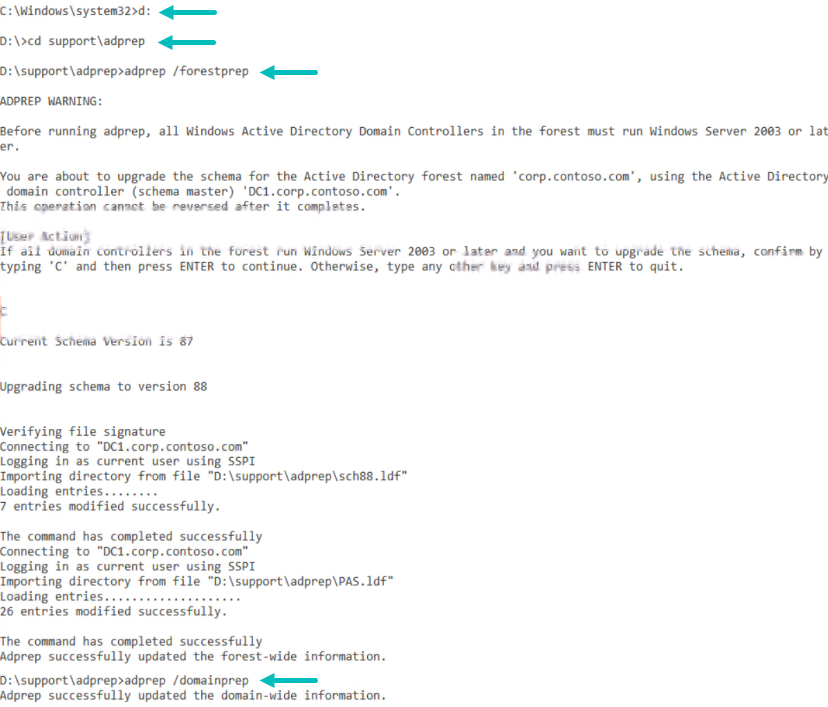
\includegraphics[width=\linewidth]{img/Methodologie/Prerequisites0.png}
	\captionsetup{width=0.9\linewidth}
	\centering		
	\caption[Preparing forest and domain ]{Preparing the forest and domain for in-place upgrade}
	\label{fig:Prerequisites}
\end{figure}
\clearpage

\subsubsection{In-place upgrade}
\label{sssec:In-place_upgrade}
After preparing the forest and domain for the in-place upgrade, the setup from the installation media is to be launched. 
From this point on, the upgrade process has been visualized in Figure \ref{fig:Inplace}. 
Be sure not to use the evaluation version of Windows Server 2019, since this does not support in-place upgrades.

\begin{figure}[h]
	\begin{subfigure}{0.5\textwidth}
		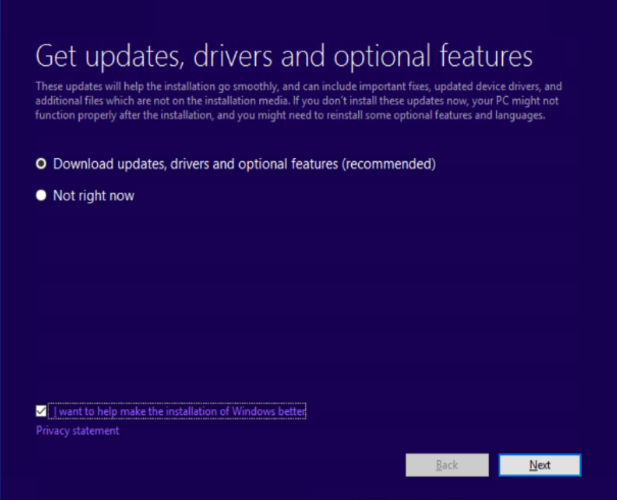
\includegraphics[width=0.9\linewidth,height=4.3cm]{img/Methodologie/InPlace0.png}
		\captionsetup{width=0.8\linewidth}
		\centering		
		\caption{Click next to migrate}
	\end{subfigure}
	\begin{subfigure}{0.5\textwidth}
		\captionsetup{width=0.8\linewidth}
		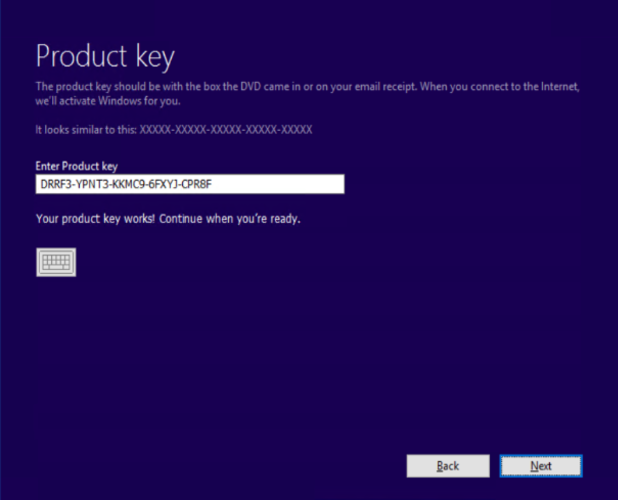
\includegraphics[width=0.9\linewidth,height=4.3cm]{img/Methodologie/InPlace1.png}
		\centering
		\caption{Enter the product key}
	\end{subfigure}
\end{figure}
\begin{figure}[h]\ContinuedFloat
	\begin{subfigure}{0.5\textwidth}
		\captionsetup{width=0.8\linewidth}
		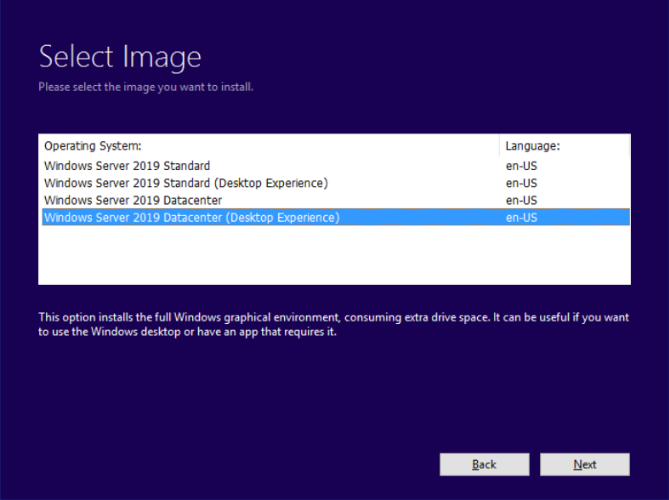
\includegraphics[width=0.9\linewidth,height=4.3cm]{img/Methodologie/InPlace2.png} 
		\centering
		\caption{Select a version of choice}
	\end{subfigure}
	\begin{subfigure}{0.5\textwidth}
		\captionsetup{width=0.8\linewidth}
		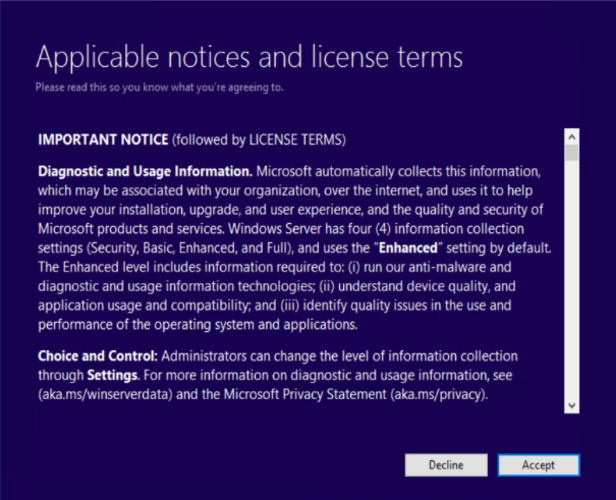
\includegraphics[width=0.9\linewidth,height=4.3cm]{img/Methodologie/InPlace3.png}
		\centering
		\caption{Accept the licence terms}
	\end{subfigure}
\end{figure}
\begin{figure}[h]\ContinuedFloat
	\begin{subfigure}{0.5\textwidth}
		\captionsetup{width=0.8\linewidth}
		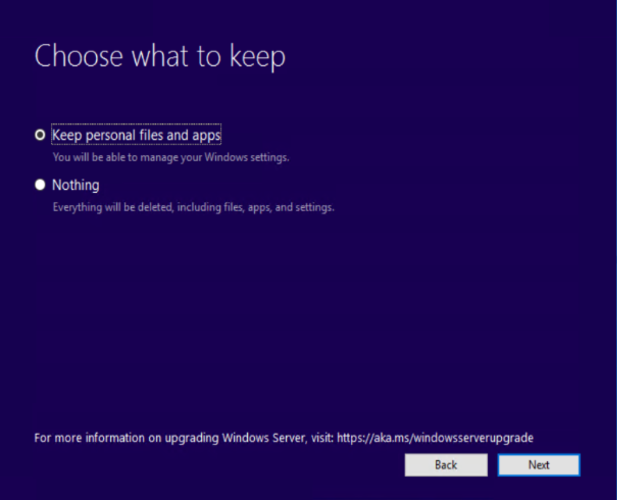
\includegraphics[width=0.9\linewidth,height=4.3cm]{img/Methodologie/InPlace4.png} 
		\centering
		\caption{Select `Keep personal files and apps` to perform an in-place upgrade}
	\end{subfigure}
	\begin{subfigure}{0.5\textwidth}
		\captionsetup{width=0.8\linewidth}
		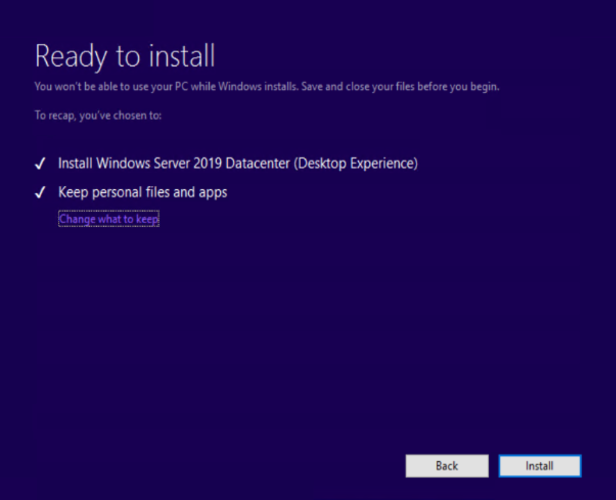
\includegraphics[width=0.9\linewidth,height=4.3cm]{img/Methodologie/InPlace5.png}
		\centering
		\caption{Review the settings and start the installation}
	\end{subfigure}
	\caption[In-place upgrade]{The in-place upgrade process}
	\label{fig:Inplace}
\end{figure}

\subsubsection{Verification}
In this paragraph, the services of the \acrshort{dc}, as well as the connection between the client and server, will be verified. 
First, the \acrfull{rdp} file will be downloaded through the \acrlong{wac}. 
Using this file, a connection to the Hyper-V \acrshort{vm} can easily be made. 
After this, the ability to log in as a domain user is verified, as the \acrshort{dc} provides the login server. 
Afterwards, the domain will be checked through the Control Panel and finally, using Powershell. 
In this final verification, the logon server will be checked as well as how the client is connected to the domain. 
It is expected that the client is connected through the recently upgraded \acrshort{dc}.
The commands, that have been used to verify this, and their expected output can be found below. 
This is also visualized in Figure \ref{fig:Verification}

\begin{lstlisting}[breaklines]
PS C:\Windows\system32> $env:LOGONSERVER
\\DC1
PS C:\Windows\system32> nltest /sc_query:corp.contoso.com
Flags: 30 HAS_IP HAS_TIMESERV
Trusted DC Name \DC1.corp.contoso.com
Trusted DC Connection Status Status = 0 0x0 NERR_Success
The command completed successfully
\end{lstlisting}

\begin{figure}[h]
	\begin{subfigure}{0.5\textwidth}
	\captionsetup{width=0.8\linewidth}
	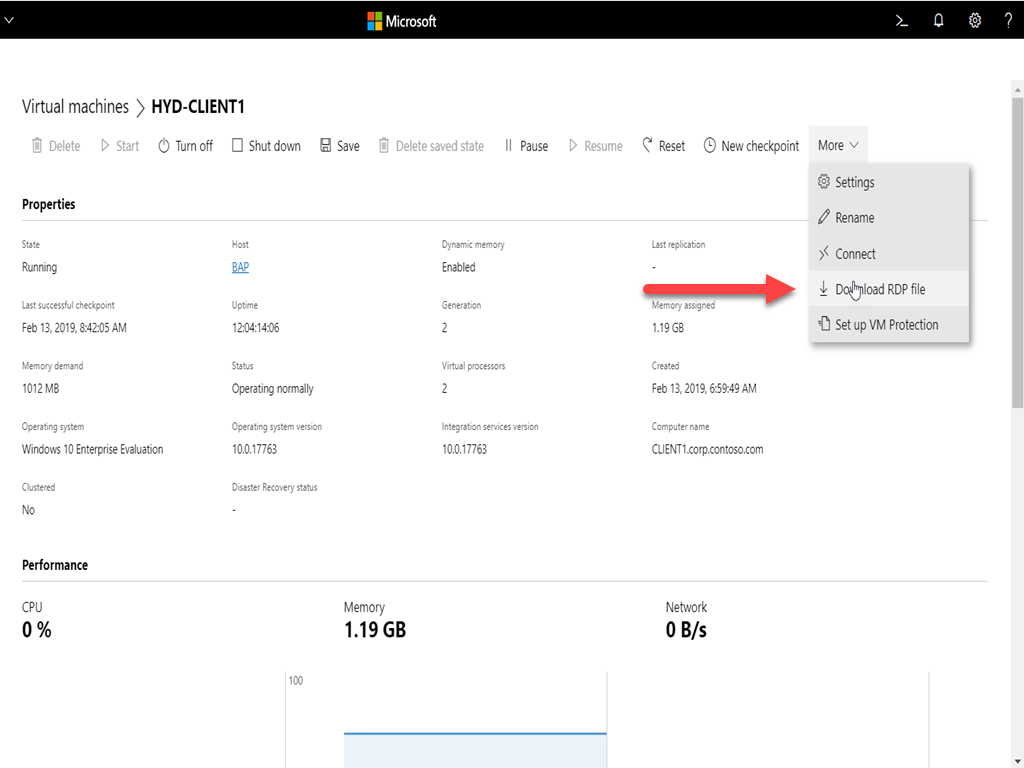
\includegraphics[width=0.9\linewidth]{img/Methodologie/Verification0.png}
	\centering
	\caption{Download and open the \acrshort{rdp} file}
\end{subfigure}
\begin{subfigure}{0.5\textwidth}
	\captionsetup{width=0.8\linewidth}
	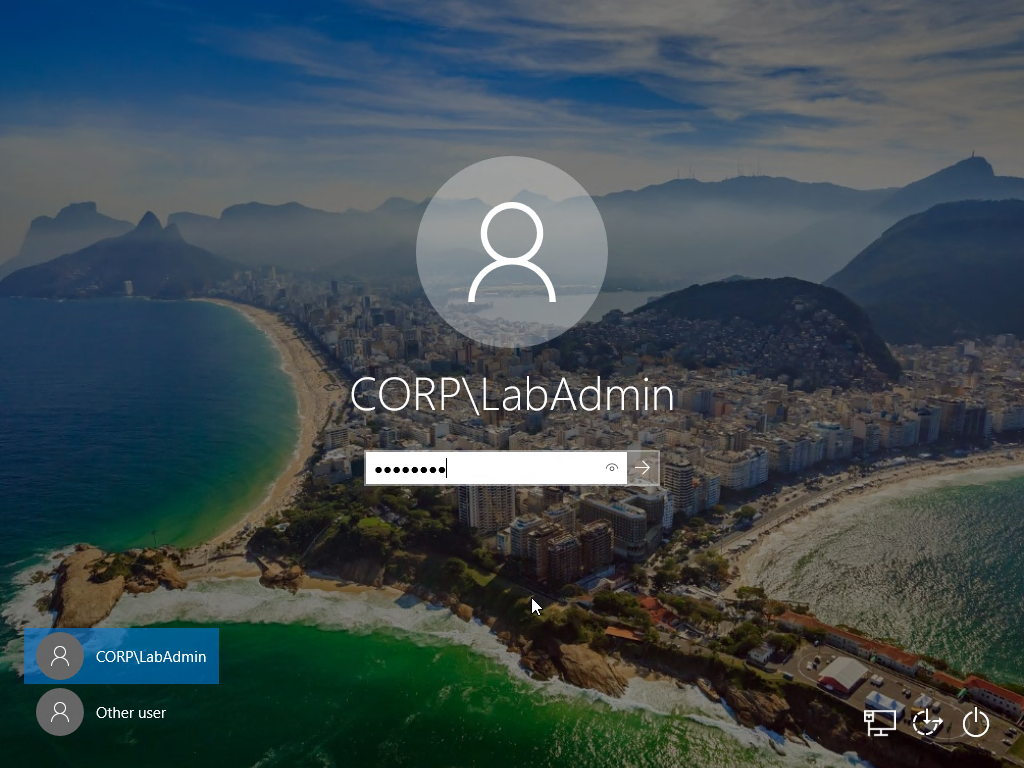
\includegraphics[width=0.9\linewidth]{img/Methodologie/Verification1.png} 
	\centering
	\caption{Log in as a domain user}
\end{subfigure}
\end{figure}
\begin{figure}[h]\ContinuedFloat
	\begin{subfigure}{0.5\textwidth}
		\captionsetup{width=0.8\linewidth}
		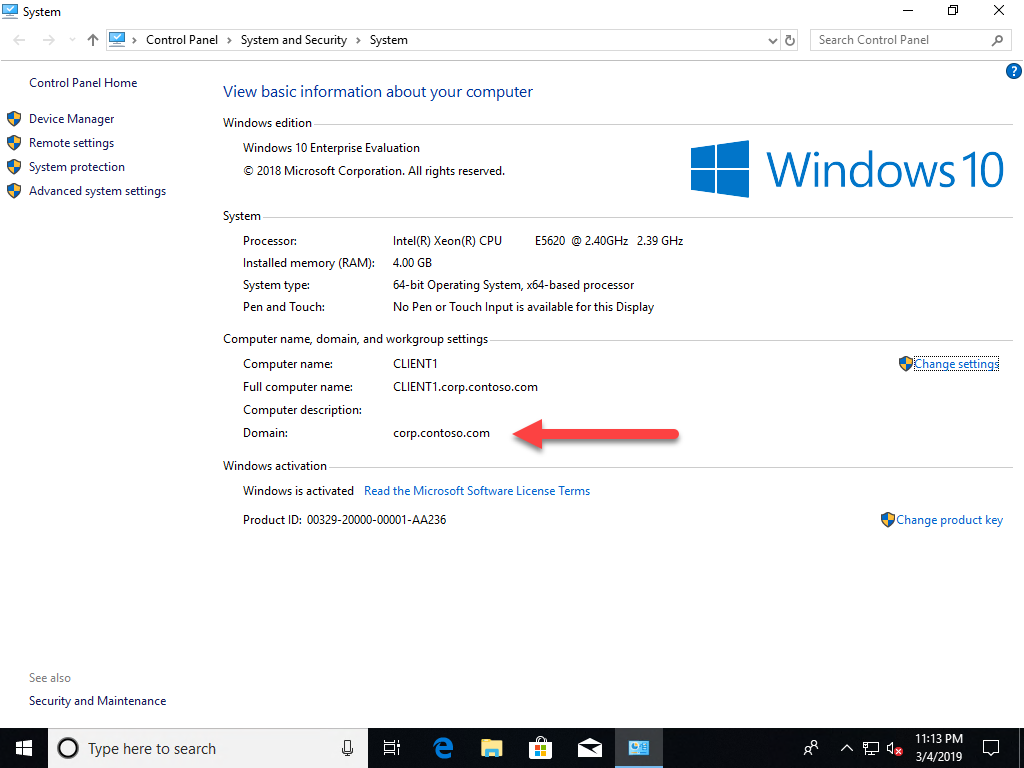
\includegraphics[width=0.9\linewidth]{img/Methodologie/Verification2.png}
		\centering
		\caption{Verify the \acrshort{dc} through the GUI}
	\end{subfigure}
	\begin{subfigure}{0.5\textwidth}
		\captionsetup{width=0.8\linewidth}
		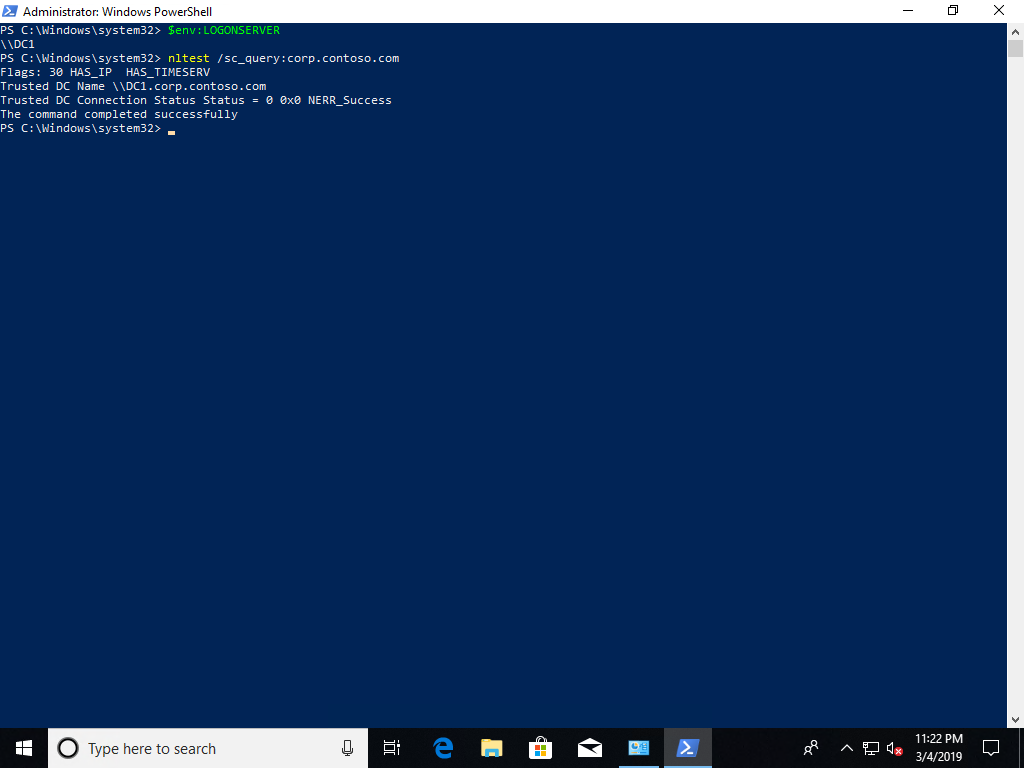
\includegraphics[width=0.9\linewidth]{img/Methodologie/Verification3.png} 
		\centering
		\caption{Verify the \acrshort{dc} through PowerShell}
	\end{subfigure}
	\caption[In-place upgrade verification]{Verifying the connection to the upgraded \acrshort{dc}}
	\label{fig:Verification}
\end{figure}
\clearpage

\subsection{Side-by-side migration to Windows Server 2019}
In this subsection, a side-by-side migration to Windows Server 2019 will be performed on the \acrshort{dc} running Windows Server 2016. 
At first, the connection between the client and the \acrshort{dc} will be verified. 
After this, the side-by-side migration will be performed by creating a new \acrshort{vm} on which Windows Server 2019 will be installed and configured. 
This \acrshort{vm} will, eventually, replace the \acrshort{dc} running Windows Server 2016. 
Finally, the connection between the new  \acrshort{dc} running Windows Server 2019 and the client will be checked.

\subsubsection{Prerequisites}
The connection between the \acrshort{dc} and the client will be verified as was done in Subsection \ref{sssec:In-place_upgrade}.
Additionally, the Windows edition will be checked. 
The prerequisites are shown in Figure \ref{fig:PrerequisitesMigration}.

\begin{figure}[h]
	\begin{subfigure}{0.5\textwidth}
		\captionsetup{width=0.8\linewidth}
		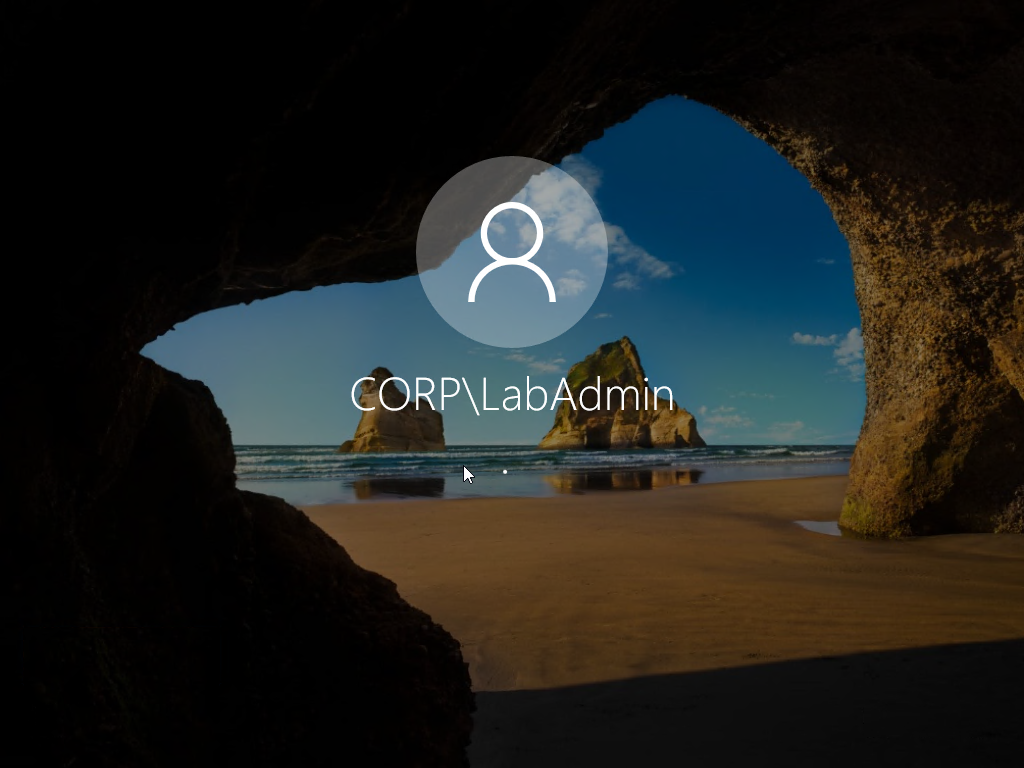
\includegraphics[width=0.9\linewidth]{img/Methodologie/Prerequisites1.png}
		\centering
		\caption{Log in as a domain user}
	\end{subfigure}
	\begin{subfigure}{0.5\textwidth}
		\captionsetup{width=0.8\linewidth}
		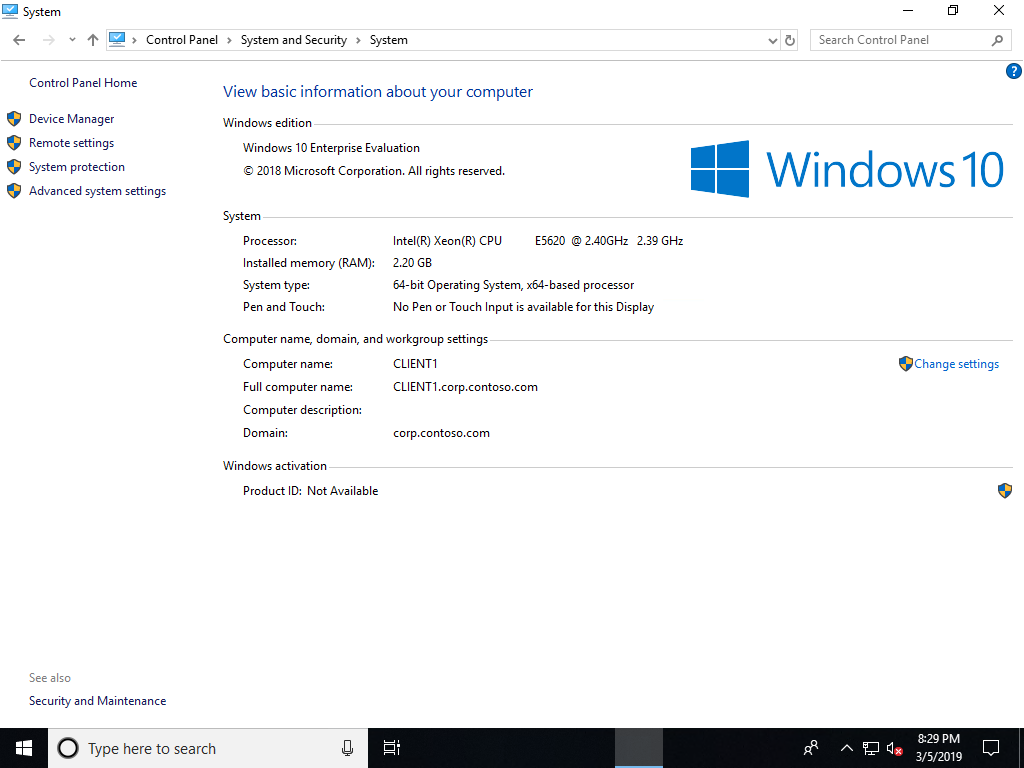
\includegraphics[width=0.9\linewidth]{img/Methodologie/Prerequisites2.png} 
		\centering
		\caption{Verify the \acrshort{dc} through the GUI}
	\end{subfigure}
\end{figure}
\begin{figure}[h]\ContinuedFloat
	\begin{subfigure}{0.5\textwidth}
		\captionsetup{width=0.8\linewidth}
		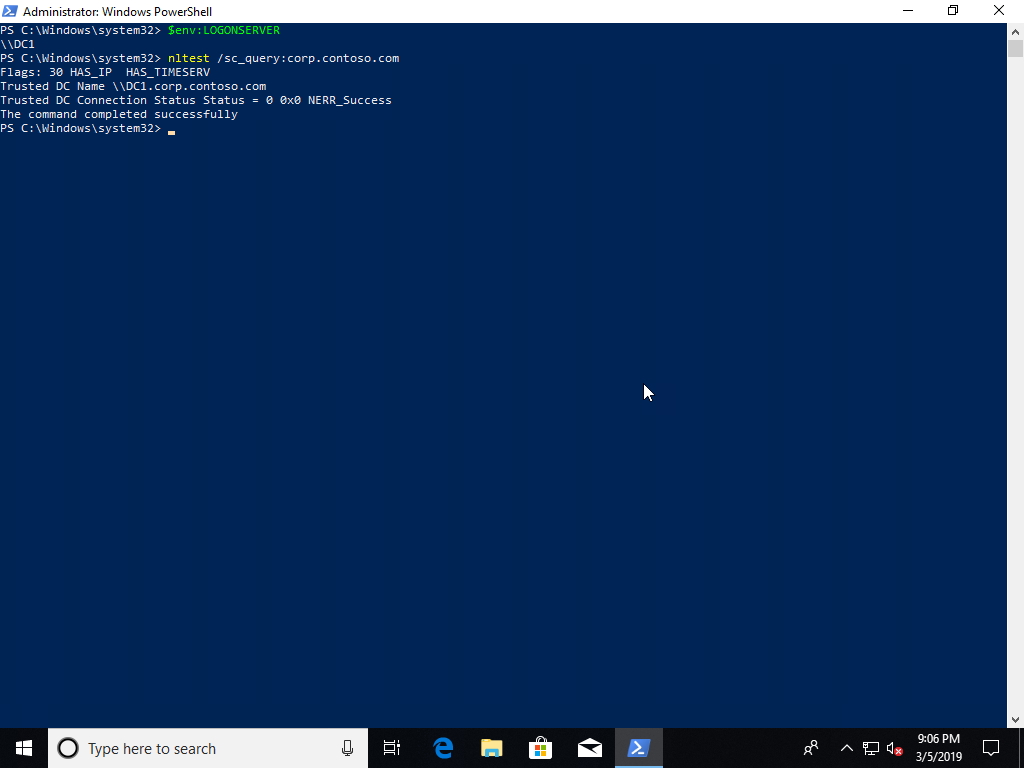
\includegraphics[width=0.9\linewidth]{img/Methodologie/Prerequisites3.png}
		\centering
		\caption{Verify the \acrshort{dc} through PowerShell}
	\end{subfigure}
	\begin{subfigure}{0.5\textwidth}
		\captionsetup{width=0.8\linewidth}
		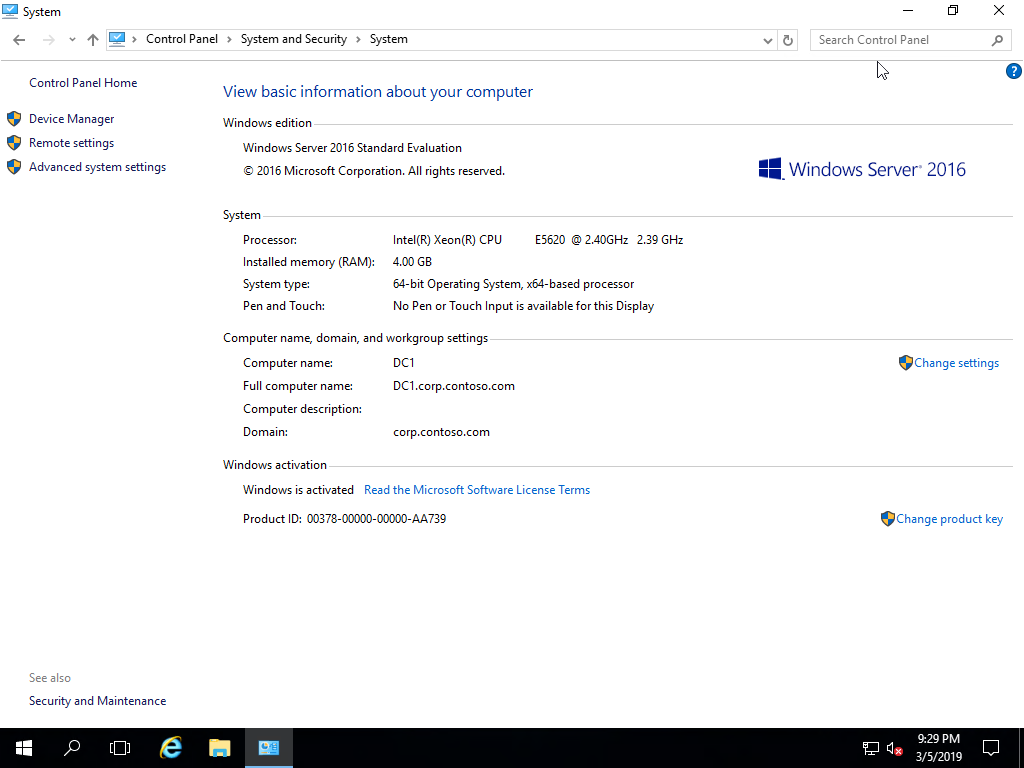
\includegraphics[width=0.9\linewidth]{img/Methodologie/Prerequisites4.png} 
		\centering	
		\caption{Verifying the Windows edition}
	\end{subfigure}
	\caption[Side-by-side migration prerequisites]{Verifying the connection between the client and \acrshort{dc}}
	\label{fig:PrerequisitesMigration}
\end{figure}

\subsubsection{Side-by-side migration}
\label{sssec:Side-by-side_migration}
The side-by-side migration to the new Windows Server 2019 \acrshort{dc}, that will be performed in this paragraph, can be divided into seven parts:
\begin{enumerate}
	\item Creating the \acrshort{vm}
	\item Installing Windows Server 2019
	\item Joining the existing domain
	\item Promoting the new \acrshort{vm} to \acrshort{dc}
	\item Migrating the FSMO roles
	\item Configuring DNS and DHCP
	\item Decommissioning the old \acrshort{dc} 
\end{enumerate}
Considering the magnitude of this side-by-side migration it is not included in the main part of this bachelor's thesis. 
However, it can be found in Appendix \ref{Migration}. 

\subsubsection{Verification}
\begin{figure}[h]
	\begin{subfigure}{0.5\textwidth}
		\captionsetup{width=0.8\linewidth}
		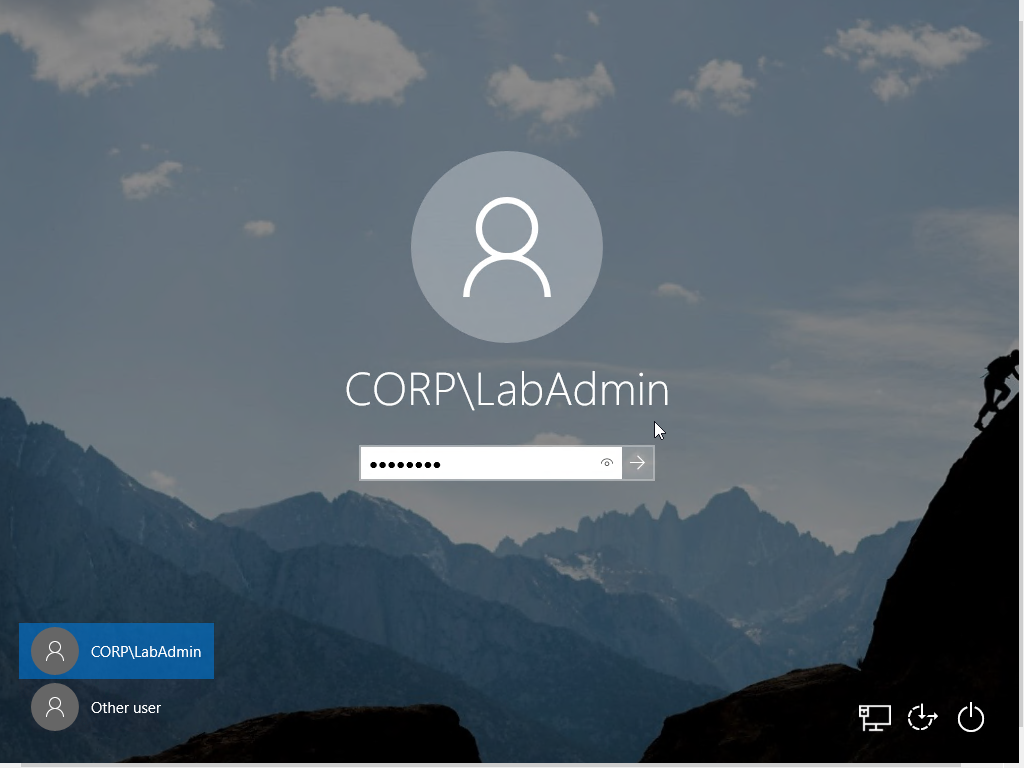
\includegraphics[width=0.9\linewidth]{img/Methodologie/Verification4.png}
		\centering
		\caption{Download and open the \acrshort{rdp} file}
	\end{subfigure}
	\begin{subfigure}{0.5\textwidth}
		\captionsetup{width=0.8\linewidth}
		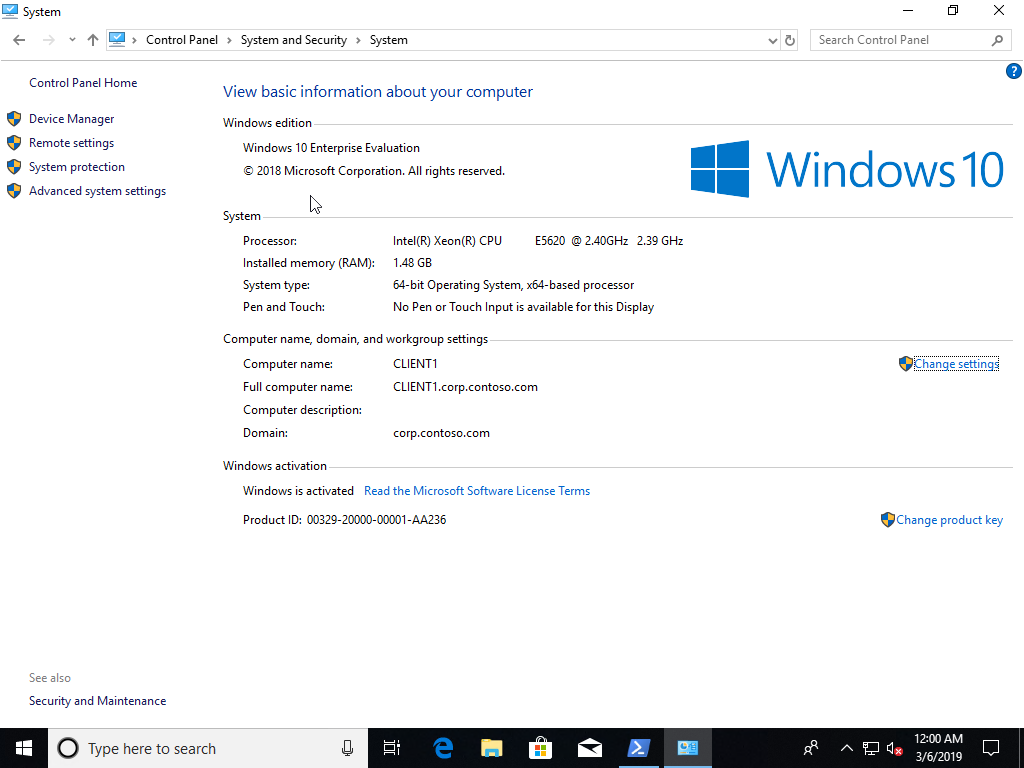
\includegraphics[width=0.9\linewidth]{img/Methodologie/Verification5.png} 
		\centering
		\caption{Log in as a domain user}
	\end{subfigure}
\end{figure}
\begin{figure}[h]\ContinuedFloat
	\begin{subfigure}{0.5\textwidth}
		\captionsetup{width=0.8\linewidth}
		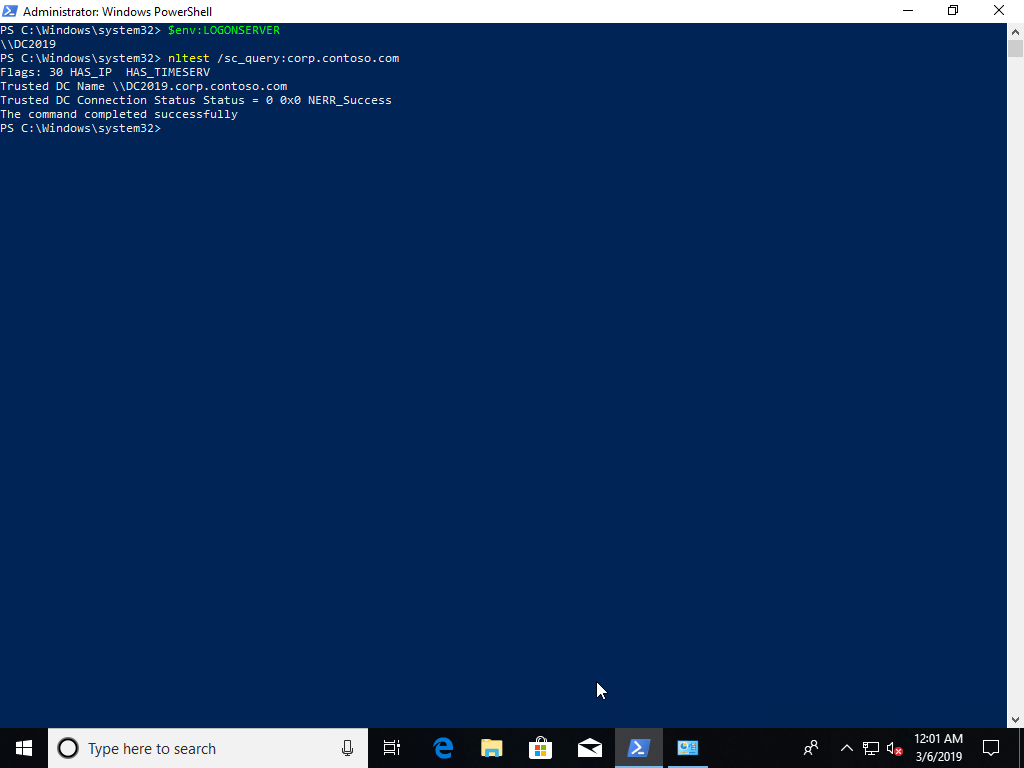
\includegraphics[width=0.9\linewidth]{img/Methodologie/Verification6.png}
		\centering
		\caption{Verify the \acrshort{dc} through the GUI}
	\end{subfigure}
	\begin{subfigure}{0.5\textwidth}
		\captionsetup{width=0.8\linewidth}
		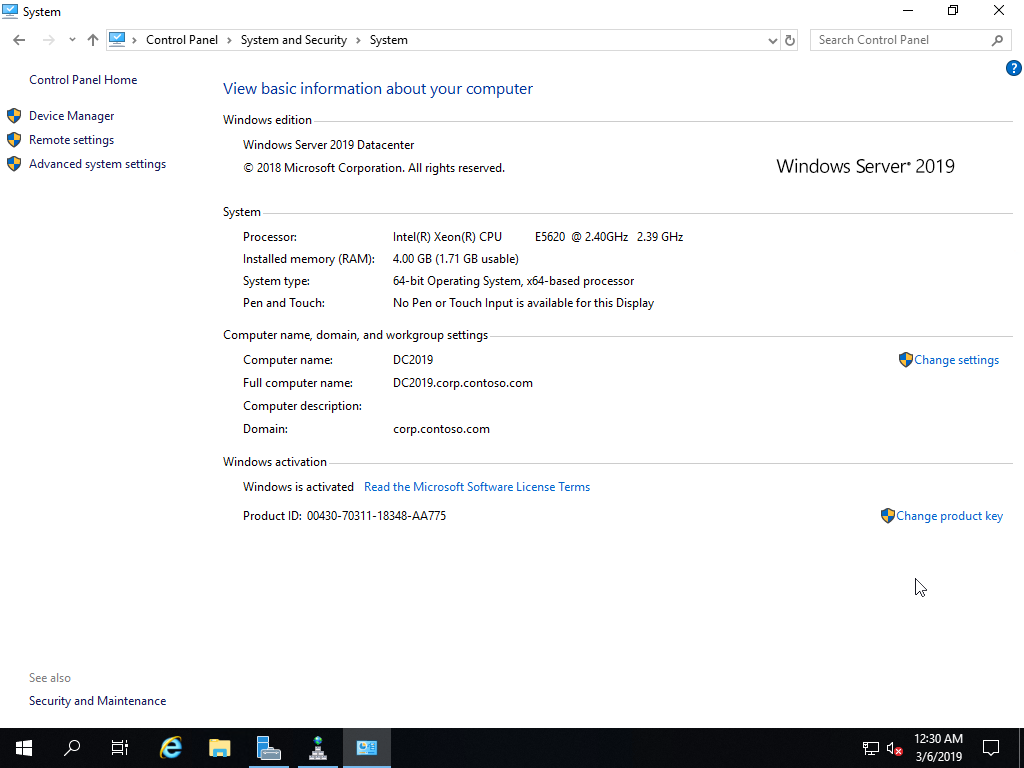
\includegraphics[width=0.9\linewidth]{img/Methodologie/Verification7.png} 
		\centering
		\caption{Verify the \acrshort{dc} through PowerShell}
	\end{subfigure}
	\caption[Verifying the side-by-side migration]{Verifying the connection to the migrated \acrshort{dc}}
	\label{fig:Migration}
\end{figure}
\clearpage

\subsection{Conclusion}
After performing the migration from Windows Server 2016 to Windows Server 2019 using both methods, either of them has its own advantages and disadvantages. 
While an in-place upgrade may seem easier to perform at first glance, it is important to remember that every \acrshort{os} has a certain amount of baggage.
Using this technique, these unnecessary files, such as old uninstallers and temporary files, will be transferred from the previous installation to the new one. 
This eventually can have an impact on the performance of the \acrshort{os}. 
It is also important to keep in mind that even though an in-place upgrade might be easier, it cannot be performed from every version to Windows Server 2019.
\\
Using the in-place upgrade from older versions of the \acrshort{os} might require the process to be repeated multiple consecutive times. 
These all increase the additional baggage that gets transferred. 
When choosing for a side-by-side migration this is not the case. 
Only the necessary files and services get transferred to the new \acrshort{os}. 
When choosing for this approach, the old infrastructure or \acrshort{vm} can be kept online so that in case of failure everything remains operational. 
Only after extensive testing, the old infrastructure can be taken offline, so that it gets replaced by the newer one. 
This provides an additional fall-back in case of any problems. 
It is important to note that the side-by-side migration currently is the only migration method that is supported for Microsoft Azure \acrshort{vm}s. 
The approach is, however, much broader and requires more research in advance. 
In this part of the proof of concept, only the \acrshort{dc} was migrated. 
This was done effortlessly thanks to the secondary \acrshort{dc}. 
The research that is required to migrate Windows Server to the latest version in a business environment will be done in the following section, for a SAP environment. 
\clearpage

\section{SAP migration}
\label{sec:SAP}
When migrating a server, it is of great importance that the is mapped in its entirety. 
This to ensure that all dependencies have been met. 
Afterwards, all of those should be verified. 
In this section, the migration from Windows Server 2016 to Windows Server 2019 will be done in a SAP environment. 
This to provide an example of the additional research that comes with the migration of a server that is performing a critical task in a business environment. 
The migration is of interest in any kind of organization for the same reasons that were mentioned before. 
Additionally, SAP recommands the usage of the latest supported version of any \acrshort{os} for its software solutions. 
Currently, the latest supported version of Windows Server is Windows Server 2019 \acrshort{ltsc}.

\subsection{Technical specifications of the SAP environment}
The proof of concept environment has been made using Microsoft Azure. 
For the environment a system running Windows Server 2016 Datacenter Edition was used.
The installation consisted of a SAP NetWeaver 7.5 ABAP stack combined with a SyBase ASE database. 
The architecture of the SAP environment can be seen in Figure \ref{fig:SAPInfra}.
The installation and configuration of the SAP environment can be found in Appendix \ref{SAPConfig}.

\begin{figure}[h]
	\captionsetup{width=0.8\linewidth}
	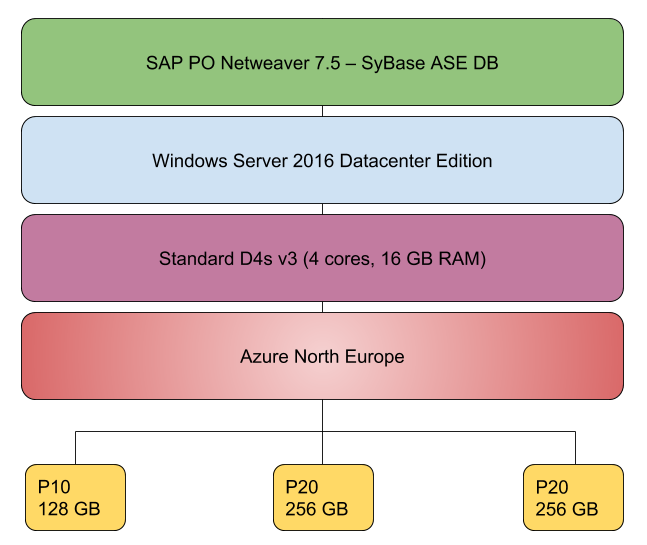
\includegraphics[width=0.9\linewidth]{img/Methodologie/SAP_PO.png}
	\centering
	\caption[SAP Infrastructure]{Infrastructure of the SAP environment}
	\label{fig:SAPInfra}	
\end{figure}

\subsection{Migration of the SAP environment}
Since Windows Server 2019, SAP offers support for full upgrades. 
This means that for non-clustered systems the in-place upgrade method is supported.
However, the traditional method of migration, using a side-by-side migration, is still supported. 
Many parts of the migration process that was described in Section \ref{sec:Migrating_the_OS} are applicable to the current environment. 
Because of this reason, the migration of the SAP environment will be kept constraint and the focus will be on the additional chores that come with this migration.
First of all, it was verified that Windows Server 2019 was supported using the SAP \acrfull{pam}, as can be seen in Figure \ref{fig:PAM}.

\begin{figure}[h]
    \captionsetup{width=0.8\linewidth}
    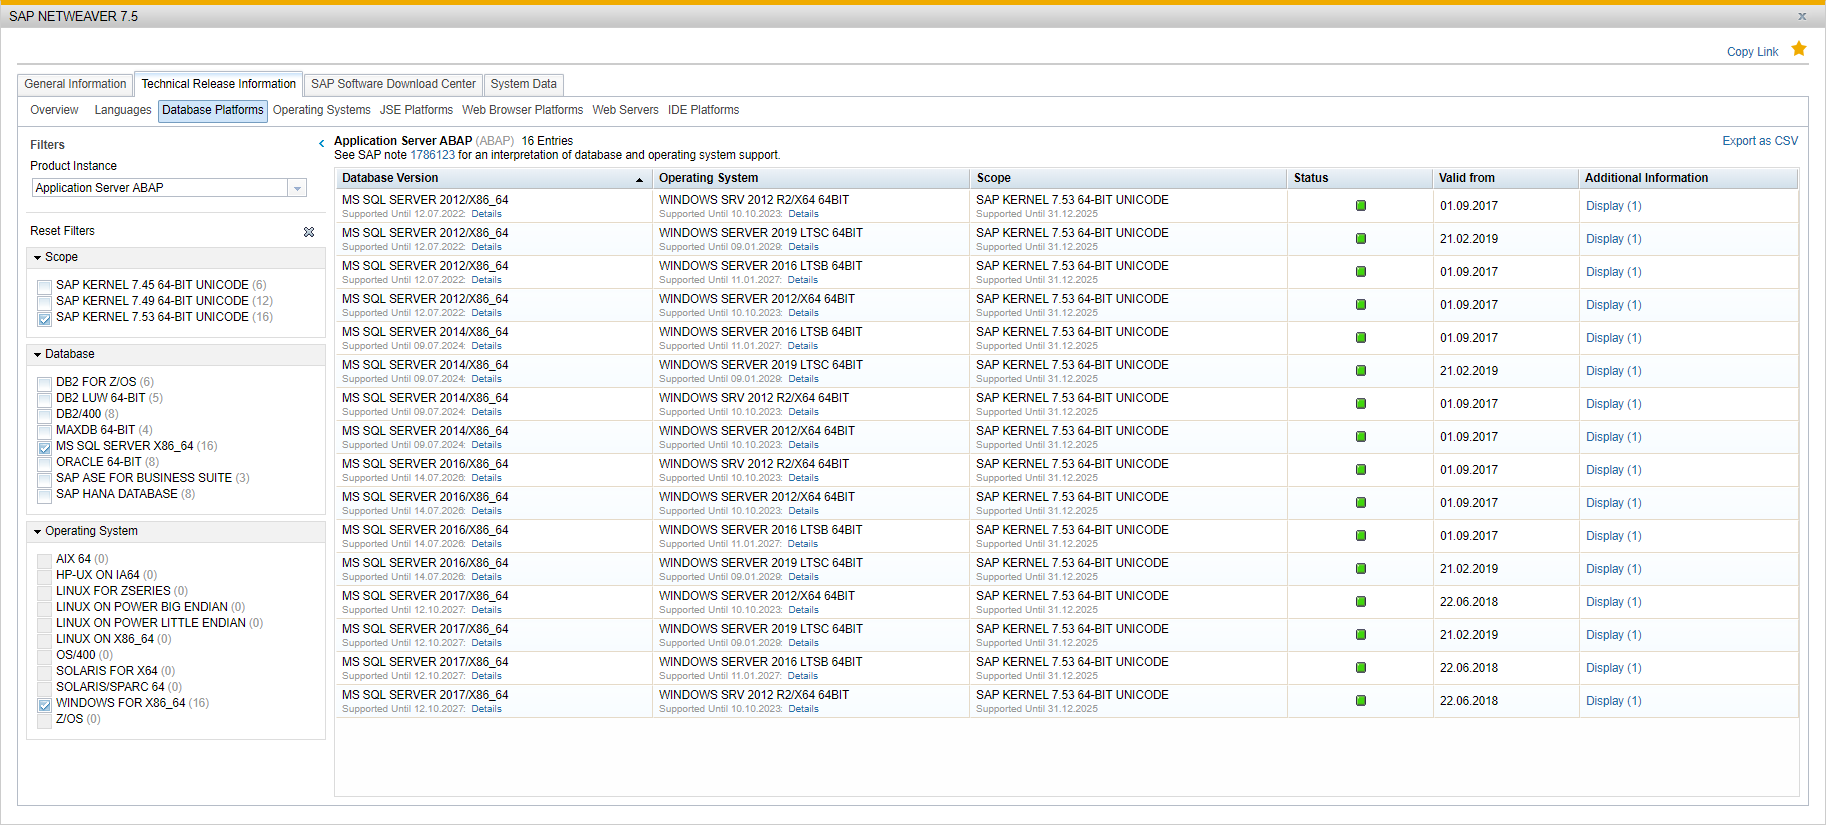
\includegraphics[width=0.9\linewidth]{img/Methodologie/PAM.png}
    \centering
    \caption[SAP \acrshort{pam}]{SAP \acrfull{pam}}
    \label{fig:PAM}	
\end{figure}

\subsubsection{Prerequisites}
\label{sssec:SAP_Prerequisites}
Before any migration, the operation of the SAP solution will be verified.  
The following process will verify the operation of the software solution.

\begin{enumerate}
    \item Browse to 'http://localhost:50013/' on the \acrshort{vm}
    \item Verify the SAP environment is running, as seen in Figure \ref{fig:SAPPreInPlace}
    \item Verify the database server as seen in Figure \ref{fig:SAPPreInPlace}
\end{enumerate}

\begin{figure}[h]
    \begin{subfigure}{0.5\textwidth}
        \captionsetup{width=0.8\linewidth}
        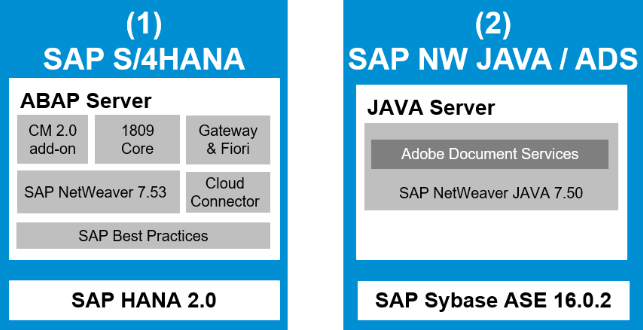
\includegraphics[width=0.9\linewidth]{img/Methodologie/SAP0.png}
        \centering
        \caption{Verify the SAP environment}
    \end{subfigure}
    \begin{subfigure}{0.5\textwidth}
        \captionsetup{width=0.8\linewidth}
        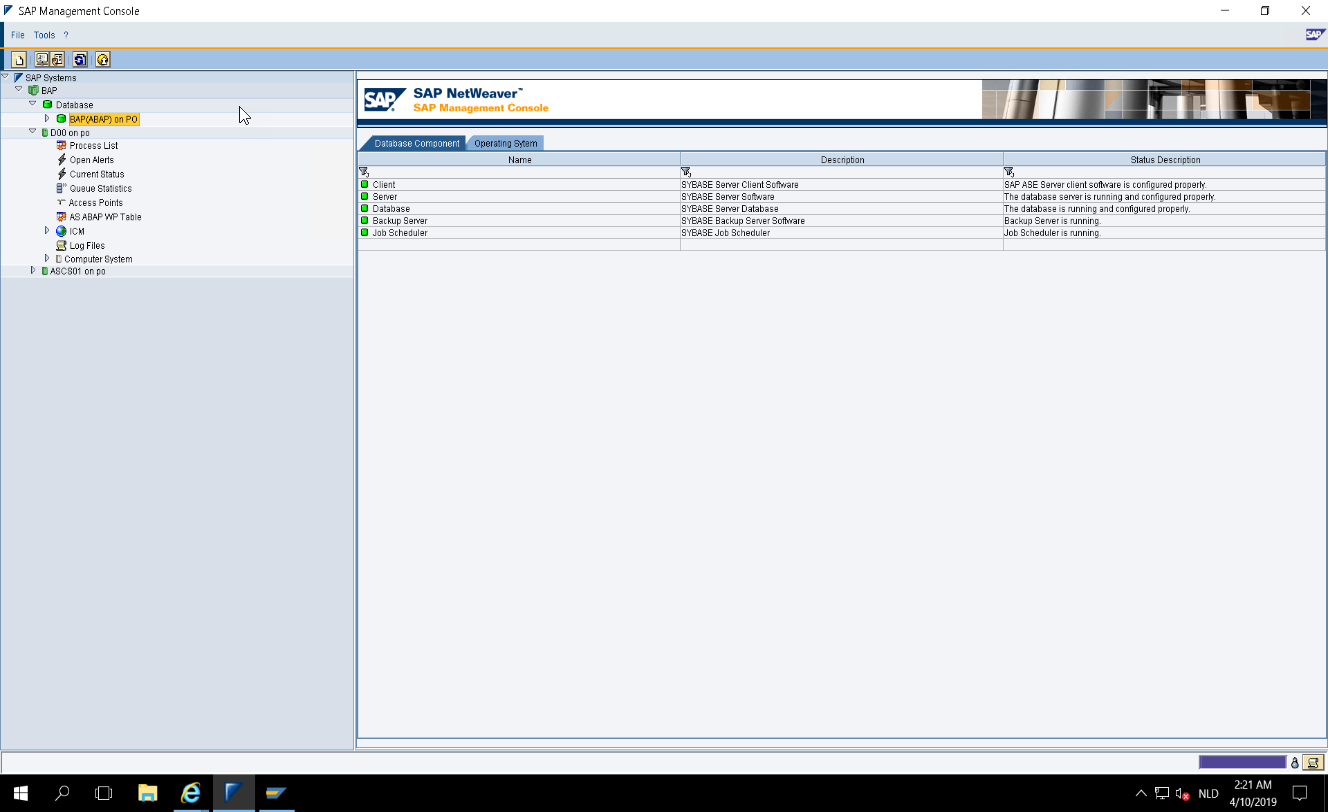
\includegraphics[width=0.9\linewidth]{img/Methodologie/SAP1.png} 
        \centering
        \caption{Verify the Database Components}
    \end{subfigure}
    \caption[Prerequisites of the in-place upgrade]{Verifying the operation through the SAP Management Console}
    \label{fig:SAPPreInPlace}	
\end{figure}
\clearpage

\subsubsection{SAP migration}
After verifying the operation of the software solution, the in-place upgrade will be performed as described in Subsection \ref{sssec:In-place_upgrade}. 
Therefore, the \acrfull{vhd} was downloaded from Azure.
The upgrade was performed through Hyper-V on the bare-metal server discussed in Section \ref{sec:Migrating_the_OS}.
Alternatively, a side-by-side migration can be performed. 
The side-by-side migration of the SAP environment can be divided into 4 parts:
\begin{enumerate}
    \item Creating the VM
    \item Installing Windows Server 2019
    \item Installing and configuring the SAP environment
    \item Backup and restore of the SyBase ASE DB
    \item Decommissioning the old SAP environment
\end{enumerate}
The first and second part of this procedure were already described in Subsection \ref{sssec:Side-by-side_migration}.
The installation and configuration has been described in Appendix \ref{SAPConfig}. 
For the third part to reduce the cut over time, the backup and restore is used followed by log shipping. 
When the last log is applied, the new system is ready to cut over. 
This way, the downtime is limited by the last log ship instead of the backup and restore of the database. 
The final part is the deletion of the old \acrshort{vm} after verifying the operation of the new \acrshort{vm}, as shown in the following paragraph.

\subsubsection{Verification}
After a successful migration, the operation of the SAP solution will be verified, as described in Subsection \ref{sssec:SAP_Prerequisites}.

\subsection{Conclusion}
After the migration of the SAP environment, it is clear that many of the aspects from the previous migration in Section \ref{sec:Migrating_the_OS} return. 
With the migration of a software solution, it is important to verify that it supports the version of the \acrshort{os} to which will be migrated beforehand. 
For SAP, this was verified using the SAP \acrshort{pam}.
In the SAP \acrshort{pam} all supported solutions can be found.
Here, all the different aspects that were installed, as described in Appendix \ref{SAPConfig}, were verified to be supported for operation on Windows Server 2019 \acrshort{ltsc}. 
Verifying the operation of all the third-party applications that need to be installed requires additional research. 
This section of the bachelor's thesis shows that no two migrations are the same. 
It emphasizes that for any migration, irrespective of the size and scope, requires its own research as no environment is identical to the other. 
There are always some variables which should be considered.  
\clearpage

\section{Base container images of Windows Server 2019}
In this final section, a comparison shall be made between the Windows, Server Core and Nano Server base container images. 
At first, the advantages of the new versions of the images will be discussed. 
This involves a comparison between version 1709 and version 1809 of the base container images. 
This will consist of comparing the size and performance of the base container images. 
Afterwards, the different use cases of the various versions will be discussed. 
These base container images have been tested in an environment as described in the following subsection.

\subsection{Technical specifications of the container environment}
The proof of concept environment for the Windows Server base container images was built using the Microsoft Azure platform. 
It uses the Standard D2s v3 (2 vcpus, 8 GB memory) Azure \acrshort{vm}, running the Windows Server 2019 Datacenter Server Core and Containers image.
The following packages will be installed inside the \acrshort{vm}:
\begin{itemize}
	\item Docker
	\item Hyper-V
	\item Windows Containers
	\item Chocolatey
	\item Git
\end{itemize}
The procedure to generate the container environment is described in Appendix \ref{Containers_Azure}.

\subsection{The advantages of version 1809}
With the arrival of version 1809, the \acrfull{sac} equivalent of Windows Server 2019, there have been improvements to the base container images. 
First, the overall size of the base container images has been significantly reduced. 
This can be seen in Figure \ref{fig:Containers}. 
The only exception is the Nano Server image, which has slightly increased in size compared to its previous version. 
This is due to the addition of new features, such as major improvements for Linux containers and container networking through Kubernetes.
The size of the different base images has been obtained by downloading and expanding them as described below. 
This was done through Windows Powershell from inside the \acrshort{vm} that was previously created on the Azure platform. 

\begin{lstlisting}[breaklines]
docker image pull mcr.microsoft.com/windows:1809
docker image pull mcr.microsoft.com/windows/servercore:1809
docker image pull mcr.microsoft.com/windows/nanoserver:1809  
docker image pull mcr.microsoft.com/windows/servercore:1709 
docker image pull mcr.microsoft.com/windows/nanoserver:1709   
docker images | Out-File .container_images.csv
Import-Csv -Path .\container_images.csv
\end{lstlisting}

\begin{figure}[h]
	\captionsetup{width=0.8\linewidth}
	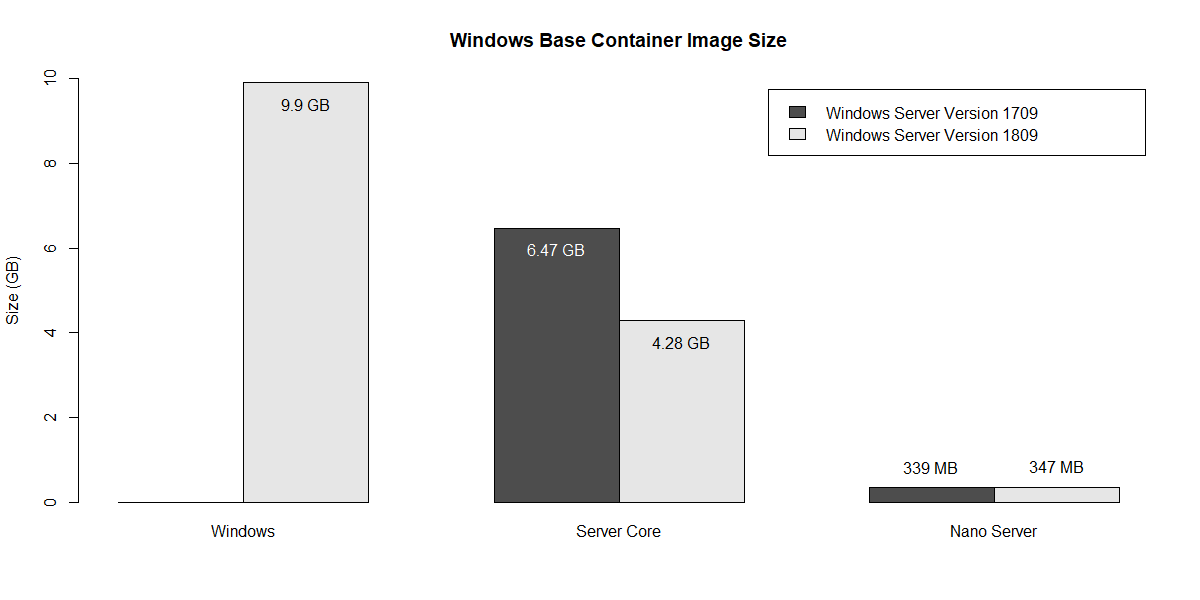
\includegraphics[width=0.9\linewidth]{img/Methodologie/Containers0.png}
	\centering
	\caption[Image size comparison]{Comparison of the Windows base container image size}
	\label{fig:Containers}	
\end{figure}

In this paragraph, the performance of the images shall be tested. 
This will be done using \href{https://benchmarkdotnet.org/}{'BenchmarkDotNet'}, a .NET library made for benchmarking. \autocite{Akinshin2019} 
Benchmarking using this library is done by calculating \acrfull{md5} and \acrfull{sha} hash functions. 
The former is mostly used in the generation of identifiers, as it is not deemed secure enough for data security. 
The latter is better suited for this but has since been improved by \acrfull{sha3}. \autocite{Enkov2017}
\\
The container will be automatically built using a Dockerfile, each of these corresponds with a base container image. 
This is needed to add the required packages inside the container to successfully perform the benchmark. 
For the Windows and Server Core base container image, these were added manually, the Nano Server base container image was provided by Microsoft. 
Following commands need to be executed on the \acrshort{vm} that was created on the Azure platform to benchmark every container individually. 
It is important to note that the kernel version of the \acrshort{os} must match the Windows image. 
While using Hyper-V isolation can circumvent this, it is not recommended since the additional virtualization of the kernel will lower the performance of the container. 
For the unambiguity of the benchmarks, Hyper-V isolation was used.

\begin{lstlisting}[breaklines]
git clone https://github.com/jensdufour/Benchmark.git
cd Benchmark	
docker build -t benchmark1 --isolation=hyperv -f .\WindowsNanoserver1709.dockerfile .
docker build -t benchmark2 --isolation=hyperv -f .\WindowsServercore1709.dockerfile .
docker build -t benchmark3 --isolation=hyperv -f .\WindowsNanoserver1809.dockerfile .
docker build -t benchmark4 --isolation=hyperv -f .\WindowsServercore1809.dockerfile .
docker build -t benchmark5 --isolation=hyperv -f .\Windows1809.dockerfile .
\end{lstlisting}

The results of running the individual benchmarks have been visualized in Figure \ref{fig:MD5} for MD5 and in Figure \ref{fig:SHA} for SHA-256. 
The figures show the average results after running the benchmarks twenty times. 
In Appendix \ref{benchmarkdata}, all the data can be found, as well as the initial results after running the benchmarks ten times. 
Eventual outliers have been removed. 
As can be seen in Figure \ref{fig:MD5} there is no significant difference in performance between the two versions of Nano Server and Server Core.
It is important to note that version 1709 was more performant in this benchmark. 

\begin{figure}[h]
	\captionsetup{width=0.8\linewidth}
	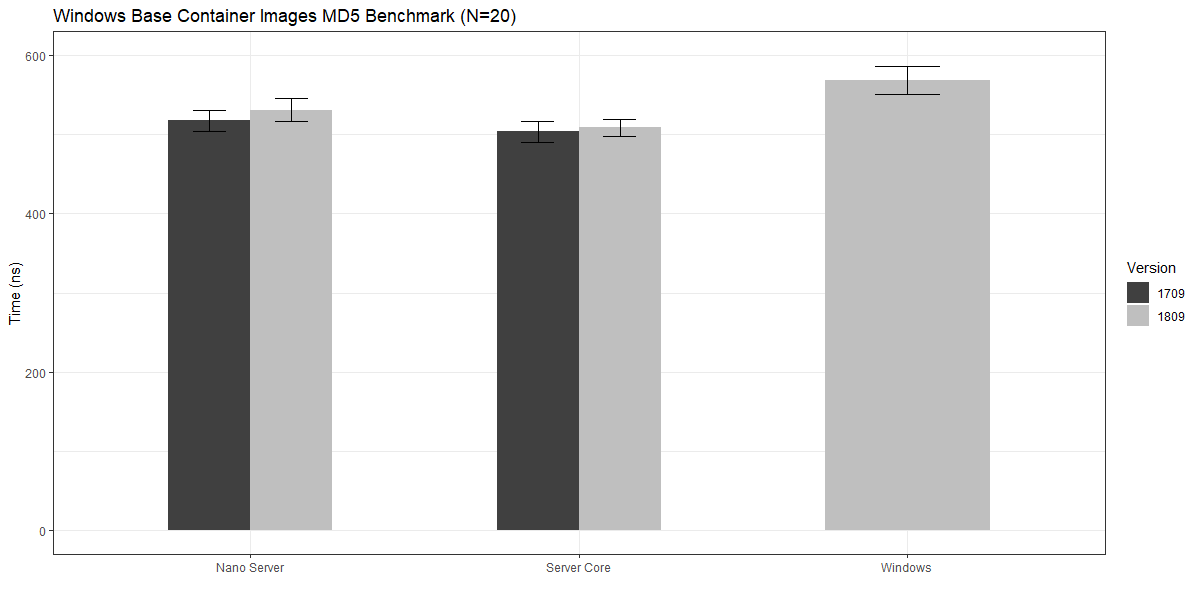
\includegraphics[width=0.9\linewidth]{img/Methodologie/Containers1.png}
	\centering
	\caption[MD5 benchmark]{Windows Base Container Image MD5 benchmark (N=20)}
	\label{fig:MD5}
\end{figure}

In Figure \ref{fig:SHA} similar results can be found. 

\begin{figure}[h]
	\captionsetup{width=0.8\linewidth}
	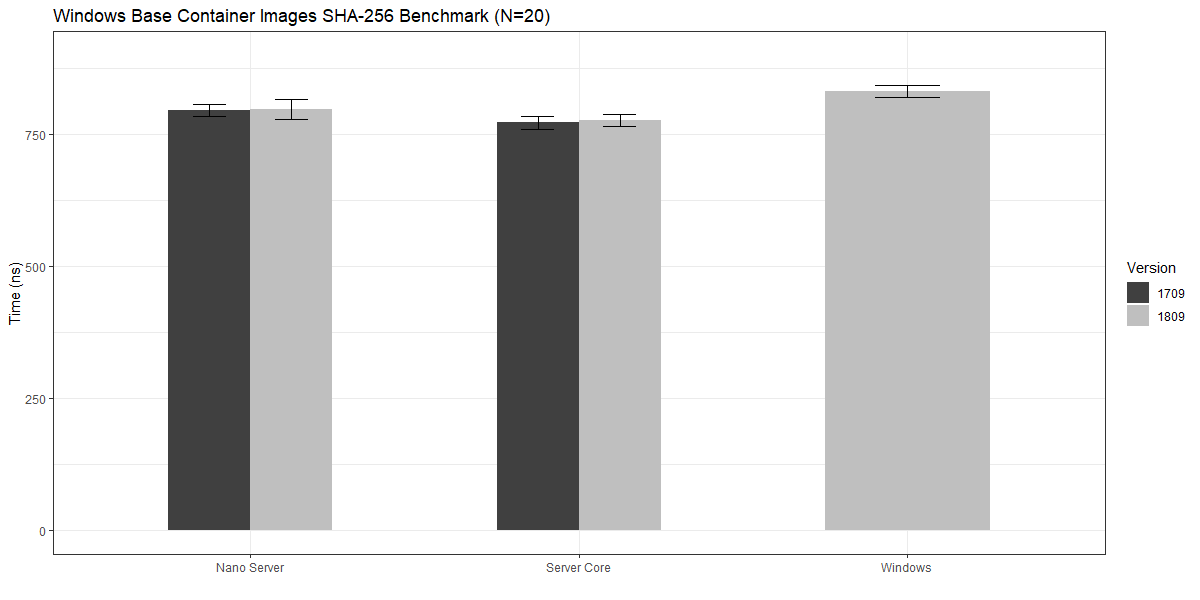
\includegraphics[width=0.9\linewidth]{img/Methodologie/Containers2.png}
	\centering
	\caption[SHA-256 benchmark]{Windows Base Container Image SHA-256 benchmark (N=20)}
	\label{fig:SHA}
\end{figure}

 When looking at the result of the benchmarks of Server Core and Nano Server, the performance of both versions is along the same lines. 
 However, the overall reduction in size and the additional features that have been added, as discussed in Chapter \ref{ch:stand-van-zaken}, make a strong case for the deployment of the latest images, version 1809. 
 The latest release of the base container images also included the Windows base container image. 
 This base container image opens a whole array of new possibilities. 
 The use case of this one and the others will be discussed in the following subsection.

\subsection{Use cases of Windows, Server Core and Nano Server}
The smallest one offered, is the Nano Server. 
This image is aimed at rapid and lightweight deployment using containers. 
It has been specifically designed for 'born in the cloud' applications. 
This is a term that has multiple usages, it refers to applications that are not legacy products. 
Applications that provide an agile deployment and offer on-demand availability. 
It is in no way meant to run typical Windows services. 
The bigger brother of Nano Server, Server Core, is more suited for this. 
This image offers application compatibility and has a wide array of built-in Windows roles and features. 
On top of this, it has full .NET Framework support instead of the basic .NET Core that is offered by the Nano Server. 
The final image that is offered is the new kid on the block. 
The Windows base container image offers almost all the Windows components in a lightweight package. 
This makes it exceptionally useful for automated \acrshort{ui} tests as it also has DirectX graphics capabilities. 
It also includes a lot of dependencies which make it usable with out-of-date applications which won't be supported in the latest version of Server Core and Nano Server. 
\\
Thanks to the further development to these base container images, their footprint has been reduced significantly. 
Although older containers from Windows Server 2016 can still run through Hyper-V isolation on Windows Server 2019, it is recommended to rebuild them with the latest available images.





% Eigen hoofdstukken
% !TeX spellcheck = en_GB
%%=============================================================================
%% Toekomstvisie
%%=============================================================================

\chapter{\IfLanguageName{dutch}{Toekomstvisie}{Future vision}}
\label{ch:toekomstvisie}
% TODO
\section{Microsoft Azure}
\section{\acrfull{wac}}


% !TeX spellcheck = en_GB
%%=============================================================================
%% Conclusie
%%=============================================================================

\chapter{\IfLanguageName{dutch}{Conclusie}{Conclusion}}
\label{ch:conclusie}

% TODO: Trek een duidelijke conclusie, in de vorm van een antwoord op de
% onderzoeksvra(a)g(en). Wat was jouw bijdrage aan het onderzoeksdomein en
% hoe biedt dit meerwaarde aan het vakgebied/doelgroep? 
% Reflecteer kritisch over het resultaat. In Engelse teksten wordt deze sectie
% ``Discussion'' genoemd. Had je deze uitkomst verwacht? Zijn er zaken die nog
% niet duidelijk zijn?
% Heeft het onderzoek geleid tot nieuwe vragen die uitnodigen tot verder 
% onderzoek?

%BAP is waarom het te doen, niet hoe het te doen!!!
%Ook Azure voor de toekomst vernoemen, hoe kan dit on-premise vervangen
%%=============================================================================
%% Bijlagen
%%=============================================================================
\appendix
\renewcommand{\chaptername}{Appendix}
%%---------- Onderzoeksvoorstel -----------------------------------------------
\chapter{Research proposal}
The subject of this bachelor's thesis is based on a research proposal that has been assessed in advance by the promoter. This proposal is included in this appendix.
% Verwijzing naar het bestand met de inhoud van het onderzoeksvoorstel
% !TeX spellcheck = en_GB
%---------- Introduction  ---------------------------------------------------------
\section{Introduction}\label{sec:introduction}
Windows Server is a well-known \acrfull{os} among \acrfull{it} professionals. With major organizations all around the globe, like Infosys, that have implemented some form of the \acrshort{os} in their infrastructure. \autocite{S.Chauhan2015}
One of the tasks that often need to be performed on the \acrshort{os}, is keeping applications up-to-date. 
However, it is not often described how to migrate to a newer version.  
This does not mean that frequent updates are not important for both the addition of new features as well as the improvement of security, as this is becoming one of the big concerns of this century. 
This bachelor's thesis will go in-depth about the advantages and disadvantages of migrating to the latest version of Windows Server.
In specific, this bachelor's thesis looks at the migration from Windows Server 2016 to Windows Server 2019, with as an optional requirement the migration of a SAP environment, as this is applicable to the business environment of the originator, delaware.
The key purpose is to find a procedure that is efficient, minimizes possible downtime and is applicable not only to the originator, delaware but also to other organizations that find them self in the same situation and want to migrate their infrastructure to the latest version of the \acrshort{os}.
\subsection{Research question}
What are the advantages and disadvantages of a migration from Windows Server 2016 to Windows Server 2019 in a business environment?
\subsection{Sub-research question}
\begin{itemize}
	\item What are the differences between the Windows, Server Core and Nano Server base container images of Windows Server 2019?
	\item Can SAP be migrated from an existing Windows Server 2016 to Windows Server 2019 in a business environment?
	\item How can the new features of Windows Server 2019 be leveraged in the migrated infrastructure? 
\end{itemize}
%---------- State of the art ---------------------------------------------------
\section{State-of-the-art}\label{sec:state-of-the-art}
Windows Server 2019 was built on the strong foundation of Windows Server 2016 although it introduces new features. \autocite{Gerend2018}
These can be boiled down to four key themes \autocite{MWST2018}:
\begin{enumerate}
	\item Hybrid Cloud
	\item Security
	\item Application Platform
	\item  \acrfull{hci}
\end{enumerate}
In the following subsections, the essence of the above themes is discussed.
\subsection{Hybrid cloud}
One of the new features in terms of hybrid cloud is the Server Core App Compatibility Feature on Demand. \autocite{Pacquer2018}
This is an optional feature pack that was designed for the Windows Server 2019 Server Core base container image and can always be applied to the system. 
It significantly improves application compatibility by adding binaries and packages. 
Even with these added packages, the footprint of the machine will remain as small as possible. 
It achieves this by not implementing the Windows Desktop Experience GUI, it uses a lightweight GUI instead.
\subsection{Security}
Security has always been a fundamental part of any \acrshort{os}. 
With over 53.000 reported incidents and 2.216 confirmed data breaches, security is without a doubt hot topic. \autocite{Verizon2018} 
This is heavily reflected in the newest edition of Windows Server, with additions like \acrfull{wdatp}, Security with \acrfull{sdn} and Shielded Virtual Machines. 
This bachelor's thesis will also explore the additional safety mechanisms that were added.
\subsection{Application platform}
At the heart of a server, applications can be found. 
Different applications allow one server to provide multiple services for end-users. 
There have been key improvements in this aspect as well. 
These improvements are mostly virtualization and security related. 
\subsection{\acrfull{hci}}
This technology could easily come out of buzzword bingo however, it is perhaps the most exciting feature that was improved in the release of Windows Server 2019. 
\acrshort{hci} makes it effortless to scale up from two nodes to a hundred node environment. 
This makes the technology intriguing for organizations with an in-house data centre.
%---------- Methodology ------------------------------------------------------
\section{Methodology}\label{sec:methodology}
Extensive research will be done before attempting the migration. The proof of concept will consist of an environment with Windows Server 2016 that will be migrated to Windows Server 2019. This will be done both using the in-place upgrade and side-by-side migration method. By carrying out this migration, the advantages and disadvantages will become clear. \\
Carrying out the migration will show the limitations and features of the latest version. 
Afterwards, an attempt will be made to migrate an existing SAP environment to our new and optimized Windows Server 2019 environment.\\
Finally, the different Windows Base Container Images will be compared, both in terms of performance and size. 
The goal at the end of the proof of concept is to make a reasoned decision between Windows Server 2016 and Windows Server 2019.
%---------- Expected results ----------------------------------------------
\section{Expected results}\label{sec:anticipated_results}
It is expected that the proof of concept will demonstrate the advantages of the latest Windows Server and that the migration is an investment in the future. However, migrating a SAP will not yet be recommended due to the new nature of Windows Server 2019. Also, when looking at the Windows Base Container Images, the latest version will have the upper hand. 
%---------- Expected conclusion ----------------------------------------------
\section{Expected conclusions}\label{sec:anticipated_conclusions}
It is expected to conclude that migration from Windows Server 2016 to Windows Server 2019 is perfectly manageable, with a preference for a full migration,  however additional research will be necessary for each individual software solution. 
%%---------- Andere bijlagen --------------------------------------------------
% TODO: Voeg hier eventuele andere bijlagen toe
%\input{...}
%%---------- Referentielijst --------------------------------------------------
\printbibliography[heading=bibintoc]
\end{document}